\documentclass[10pt]{article}
\usepackage[letterpaper,top=0.7in,bottom=0.8in,left=0.8in,right=0.8in]{geometry}
\usepackage[T1]{fontenc}
\usepackage[utf8]{inputenc}
\usepackage{lmodern}
\usepackage{microtype}
\usepackage{amsmath}
\usepackage{graphicx}
\usepackage{booktabs}
\usepackage{xcolor}
\usepackage{titlesec}
\usepackage{parskip}
\usepackage{fancyhdr}
\usepackage[hidelinks]{hyperref}
\usepackage{mdframed}

\graphicspath{{Figures/}}

%% Colour palette
\definecolor{P0red}{RGB}{200,40,40}
\definecolor{P1amber}{RGB}{200,130,0}
\definecolor{P2gray}{RGB}{100,100,100}
\definecolor{okgreen}{RGB}{40,140,60}
\definecolor{notebg}{RGB}{245,245,255}

%% Severity boxes
\newmdenv[backgroundcolor=P0red!15,linecolor=P0red,linewidth=1pt,
          innertopmargin=4pt,innerbottommargin=4pt]{p0box}
\newmdenv[backgroundcolor=P1amber!15,linecolor=P1amber,linewidth=1pt,
          innertopmargin=4pt,innerbottommargin=4pt]{p1box}
\newmdenv[backgroundcolor=notebg,linecolor=gray!40,linewidth=0.5pt,
          innertopmargin=4pt,innerbottommargin=4pt]{notebox}

\newcommand{\Pz}[1]{\textbf{\textcolor{P0red}{[P0 — #1]}}}
\newcommand{\Po}[1]{\textbf{\textcolor{P0red}{[P0]}}}
\newcommand{\Pp}[1]{\textbf{\textcolor{P1amber}{[P1 — #1]}}}
\newcommand{\Ppp}[1]{\textbf{\textcolor{P2gray}{[P2 — #1]}}}
\newcommand{\OK}[1]{\textbf{\textcolor{okgreen}{[OK — #1]}}}

%% Section format
\titleformat{\section}{\large\bfseries}{}{0em}{}[\titlerule]
\titleformat{\subsection}{\normalsize\bfseries}{}{0em}{}
\titlespacing*{\section}{0pt}{1.0em}{0.4em}
\titlespacing*{\subsection}{0pt}{0.7em}{0.2em}

%% Header/footer
\pagestyle{fancy}
\fancyhf{}
\fancyhead[L]{\small orcast submission audit deck}
\fancyhead[R]{\small 2026-06-25}
\fancyfoot[C]{\thepage}

\setlength{\parskip}{0.35em}
\setlength{\parindent}{0pt}

\begin{document}

\begin{center}
{\Large\bfseries orcast Submission Audit Deck}\\[0.4em]
{\normalsize Gil Raitses $\cdot$ 2026-06-25 $\cdot$ Deadline: June 29, 2026 5:00 PM}\\[0.2em]
{\small Physical world model fusion for orca encounter forecasting and community platform for field researchers}
\end{center}

\vspace{0.5em}
\begin{notebox}
\textbf{How to use this deck.} Read top to bottom. Every \textbf{\textcolor{P0red}{[P0]}} item must be fixed before submission. \textbf{\textcolor{P1amber}{[P1]}} items should be fixed if time allows. \textbf{\textcolor{P2gray}{[P2]}} items are minor. Mark in the margins what you intend to fix, then execute Section 5 (Fix Checklist) in order.
\end{notebox}

\tableofcontents
\newpage

\section{Section 1: Demo Beat Audit}

Each beat shows the actual still frame captured by the Playwright walkthrough, followed by three items: what the beat is supposed to demonstrate, what a first-time judge sees, and what to fix.

% ─────────────────────────────────────────────────────────────────────────────
\subsection{Beat 01, Home (\texttt{/})}

\begin{center}
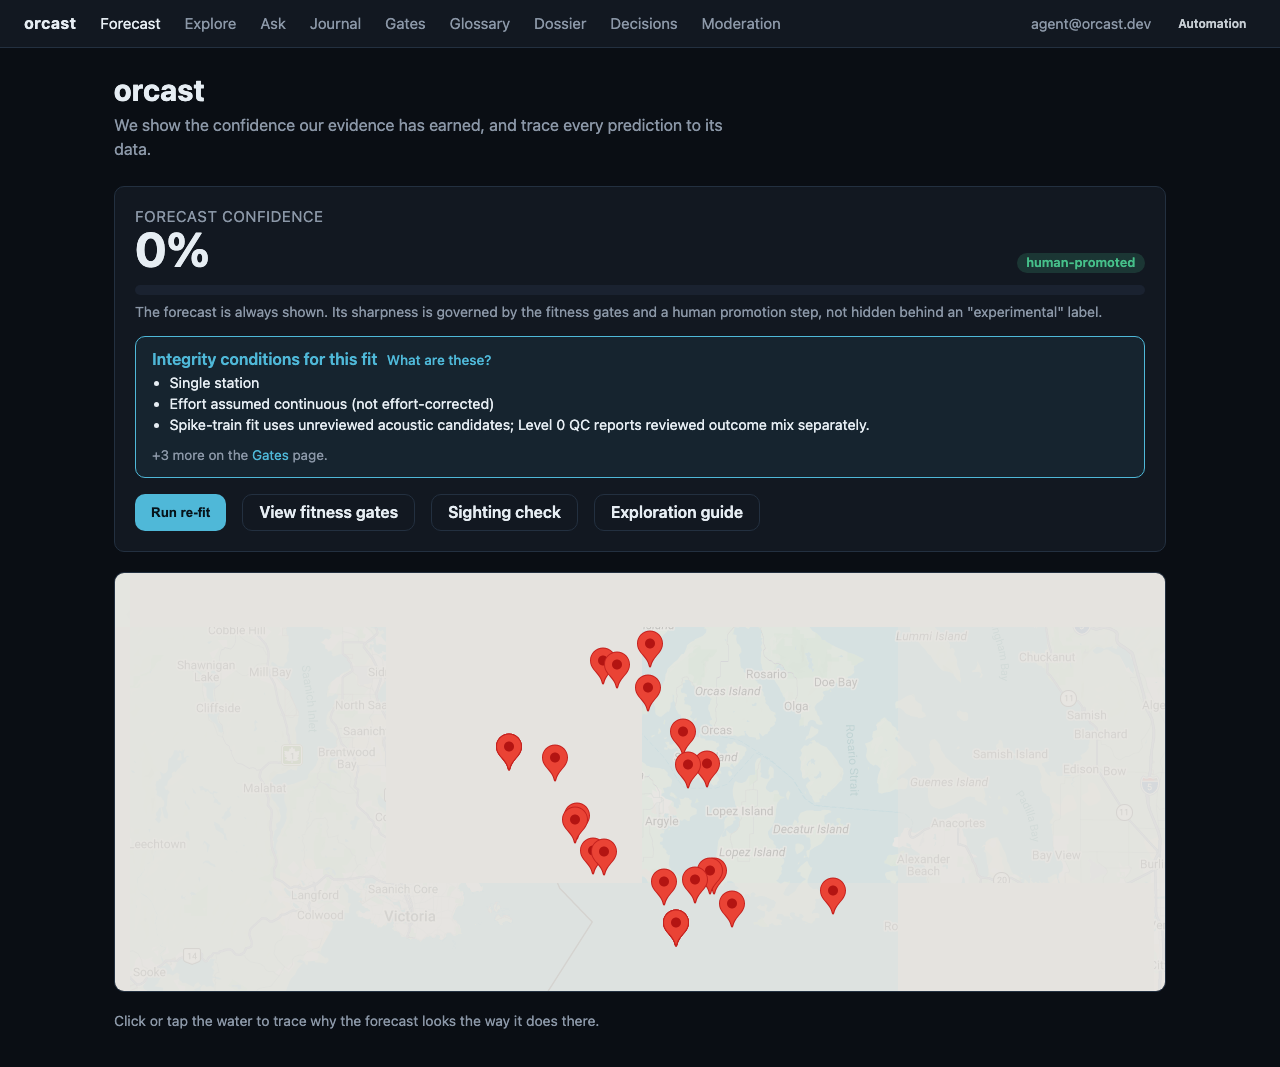
\includegraphics[width=\linewidth]{beat-01-home.png}
\end{center}

\textbf{Storyboard intent.} Establish that the system always shows the forecast but bounds the confidence it displays to what the statistical gate battery has earned. The integrity conditions block shows the model's honest self-assessment.

\textbf{What a judge sees.} A dark map with red sighting pins, a large ``0\%'' Forecast Confidence label, a list of technical caveats, and four navigation buttons. The ``Automation'' chip in the top-right corner and ``agent@orcast.dev'' are visible but small. There are no probability-coloured map cells visible, the sighting pins dominate.

\textbf{What is missing or confusing.}
\begin{itemize}
\item 0\% confidence is the correct value (no human promotion yet) but a judge reading this for the first time sees a broken product, not an honest one. The explanation is present but requires careful reading.
\item The map shows sighting pins but no hotspot confidence cells. The spatial forecast is the product, it is invisible in this frame.
\item The ``Run re-fit'' button is prominent and cyan. To a judge it reads as ``the system is not ready; please run it first.'' The button's prominence undercuts the ``always-on forecast'' claim.
\end{itemize}

\begin{p1box}
\textbf{P1, Fix before Saturday.} Pan the map to a hotspot cluster or zoom into Haro Strait so at least one confidence-coloured cell is visible before the provenance modal opens in Beat 02. Consider narrating why 0\% is the honest answer: ``No promotion has happened yet. The model fitted. The gates told it not to display high confidence. That's the product.''
\end{p1box}

% ─────────────────────────────────────────────────────────────────────────────
\subsection{Beat 02, Provenance modal}

\begin{center}
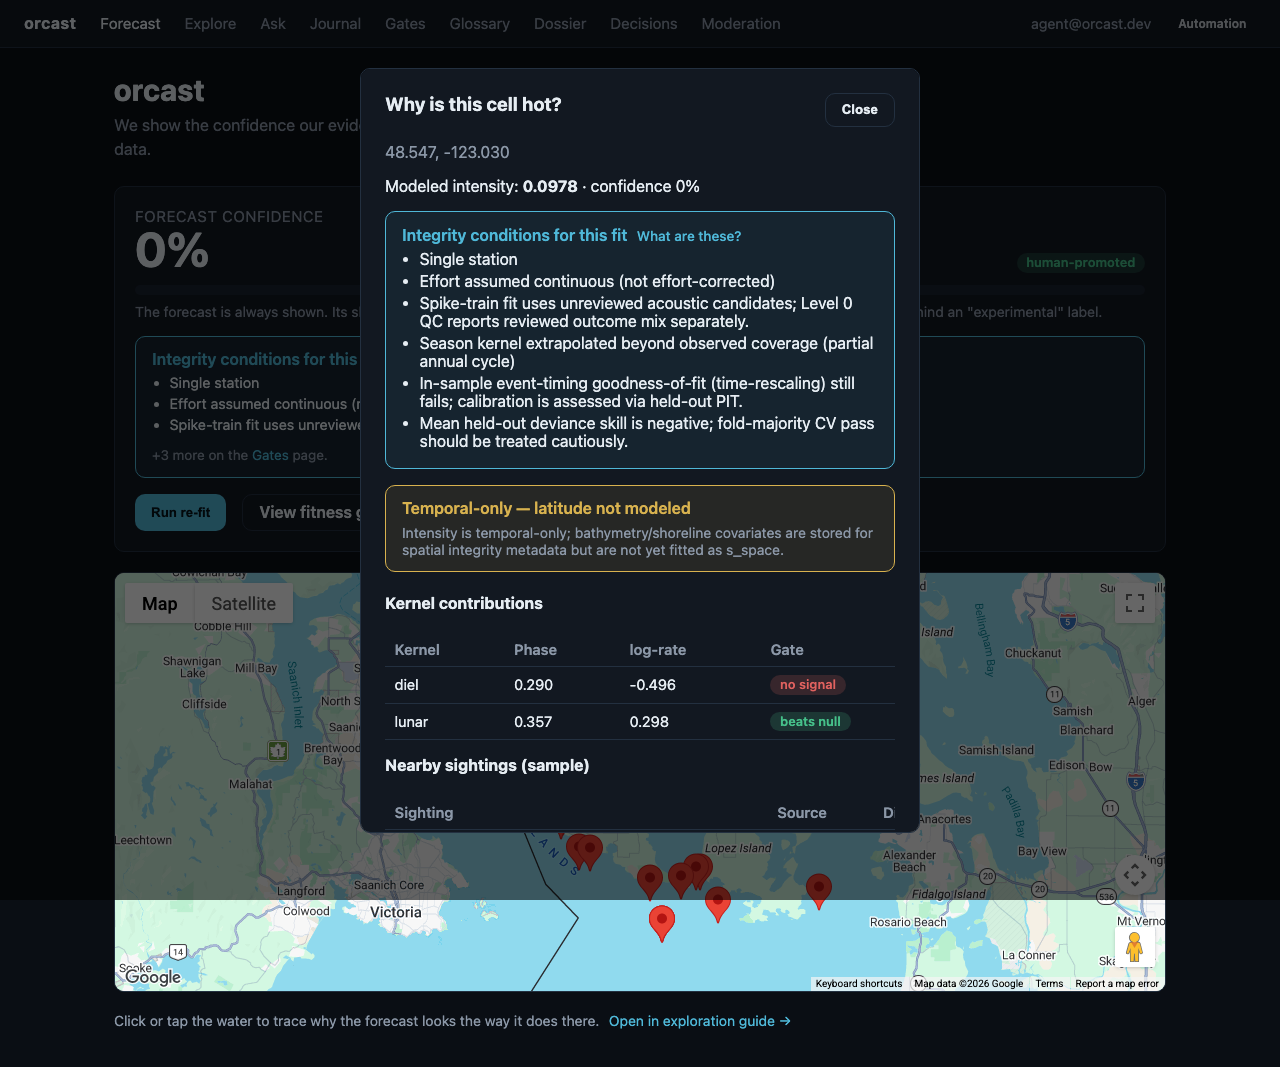
\includegraphics[width=\linewidth]{beat-02-provenance.png}
\end{center}

\textbf{Storyboard intent.} Show that every map cell traces back to its kernels, gate verdicts, and data. The provenance modal is the ``why is this cell hot?'' drilldown.

\textbf{What a judge sees.} A modal titled ``Why is this cell hot?'' over the map. Shows coordinates, modelled intensity 0.0978, confidence 0\%, six integrity conditions, a yellow ``Temporal-only, latitude not modeled'' banner, a kernel contributions table (diel: no signal; lunar: beats null), and a ``Nearby sightings'' section that is cut off.

\textbf{What is missing or confusing.}
\begin{itemize}
\item The PSTH kernel plots are blank white boxes labelled ``fixed kernel shape (offline fit artifact)''. To a judge this reads as broken image placeholders.
\item The yellow warning banner ``Temporal-only, latitude not modeled'' is alarming. It reads as a system limitation warning, not an integrity condition.
\item The modal is dense. A judge will not read six bullet-point integrity conditions in a 3-minute demo.
\end{itemize}

\begin{p0box}
\textbf{P0, Kernel PSTH plots render as blank white boxes.} This makes the product look like it has missing assets. The kernel shape images are described as ``offline fit artifacts'' which is technically accurate (they come from S3) but visually broken. Fix: either load the actual PSTH shape PNGs from S3 into the response, or remove the placeholder images and show the modulation values only.
\end{p0box}

% ─────────────────────────────────────────────────────────────────────────────
\subsection{Beat 03, Fitness gates (\texttt{/gates})}

\begin{center}
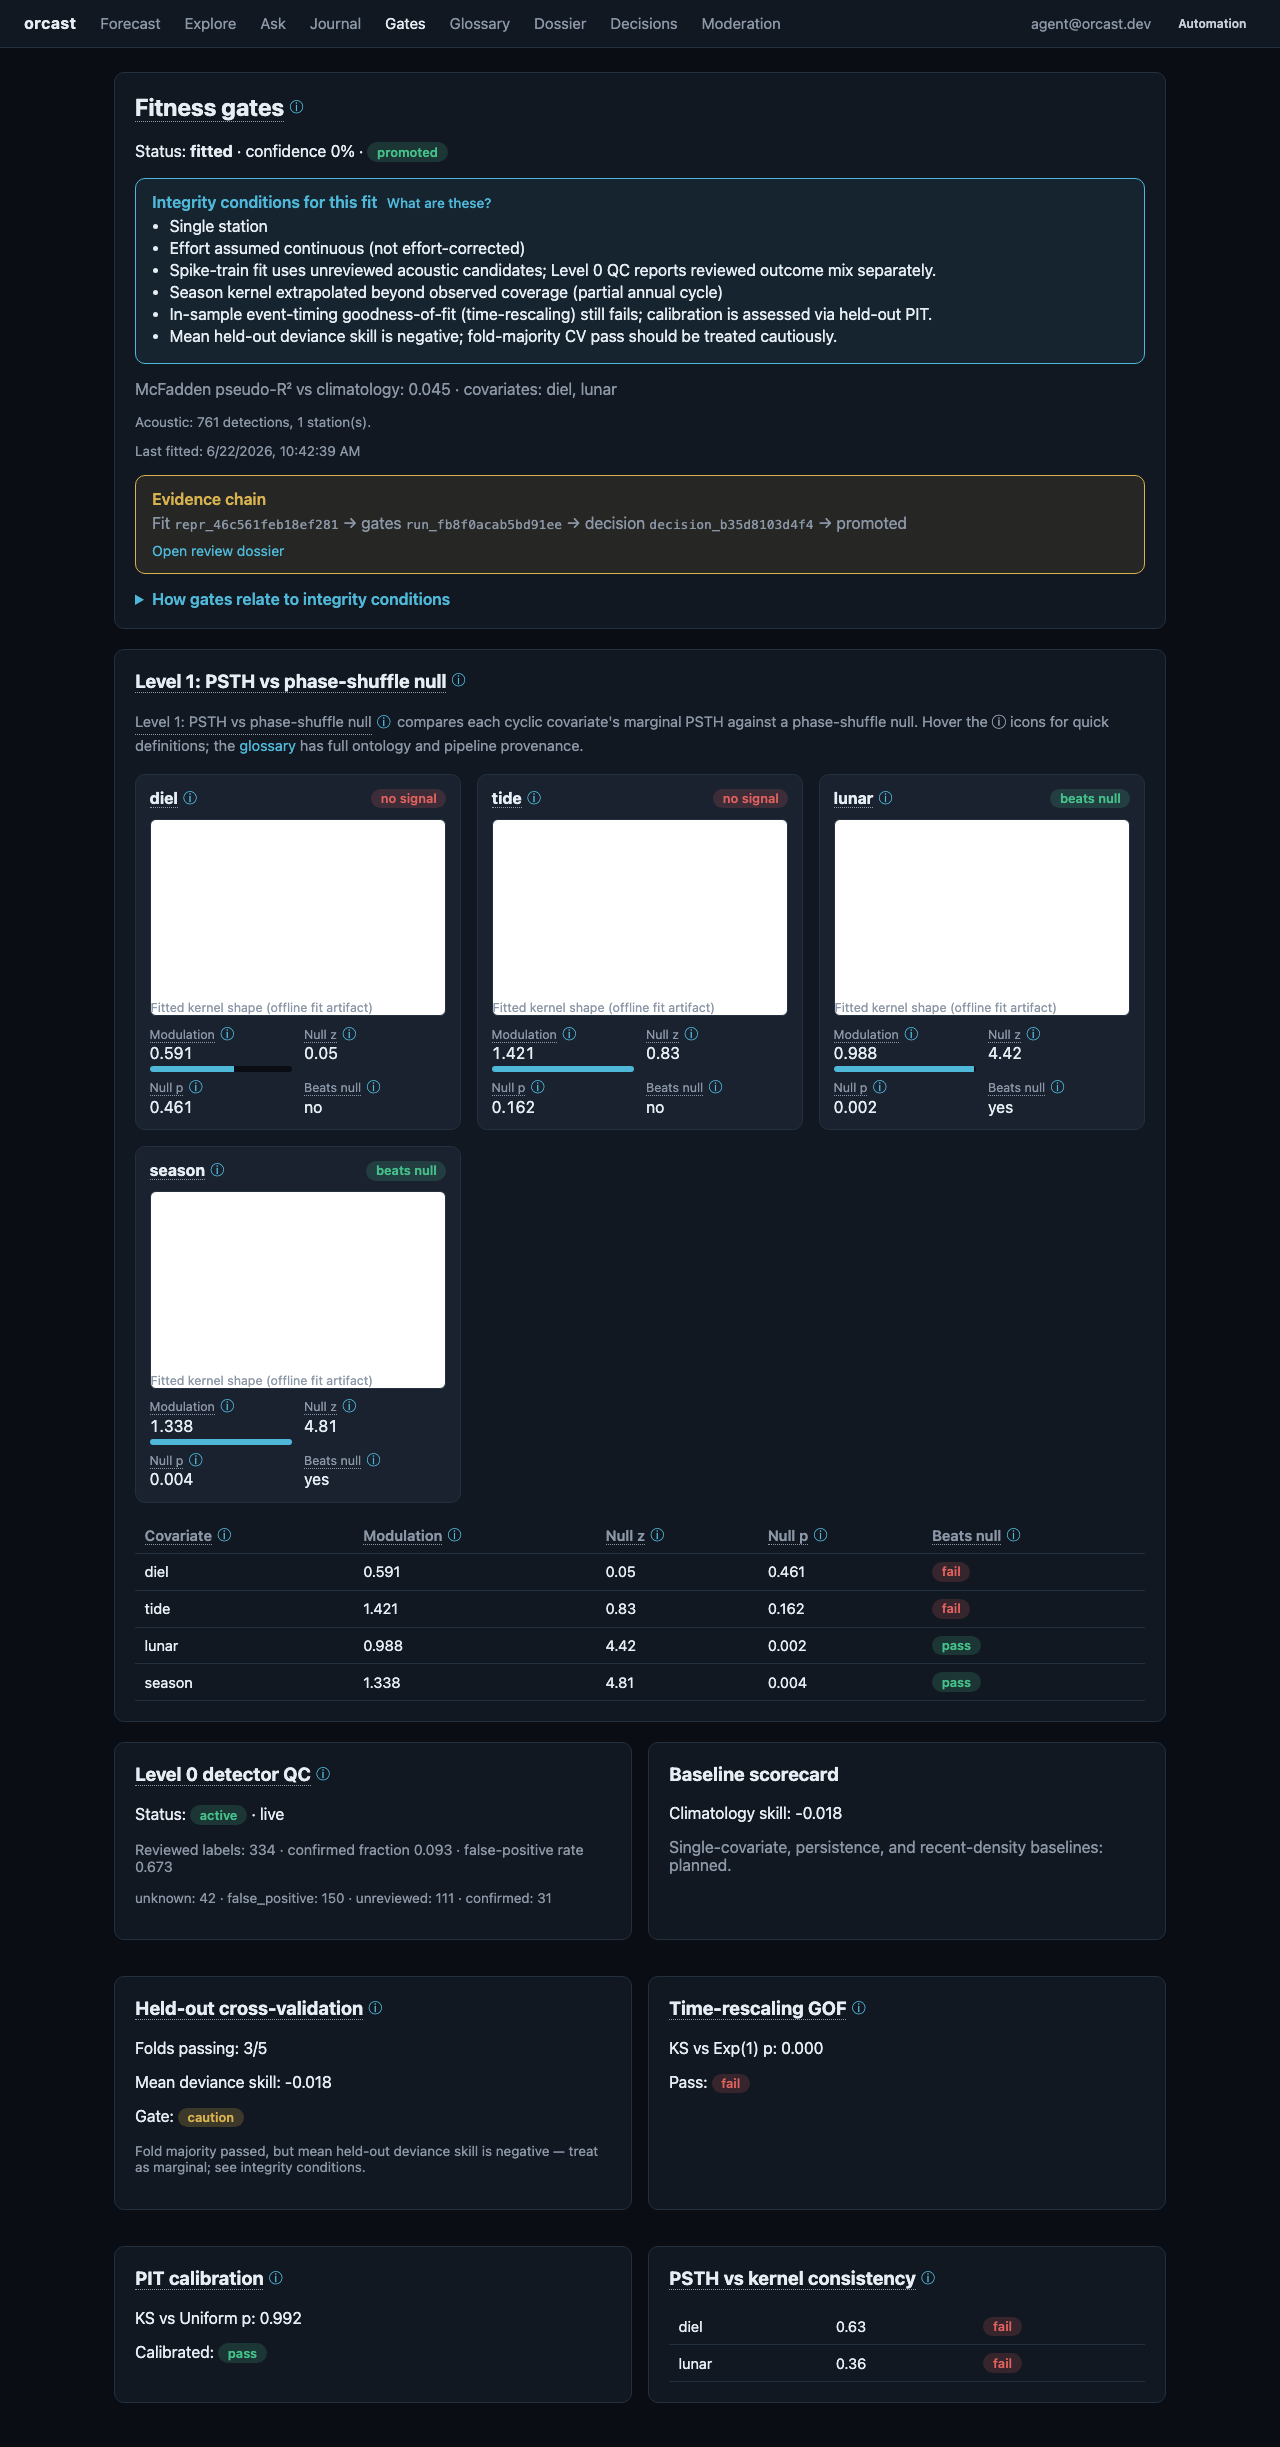
\includegraphics[width=0.75\linewidth]{beat-03-gates.png}
\end{center}

\textbf{Storyboard intent.} Show the full statistical gate battery: PSTH vs phase-shuffle null, time-rescaling goodness-of-fit, held-out cross-validation, PIT calibration. Show that the system surfaces integrity conditions rather than hiding a failing model.

\textbf{What a judge sees.} An extremely data-dense page. Status: fitted, confidence 0\%, promoted badge. Integrity conditions block. Evidence chain hash (cryptic). Level 1: four kernel panels, all showing blank white PSTH plots with modulation values below. Gate table showing diel/tide fail (red), lunar/season pass (green). Level 0 QC scorecard. CV: 3/5 folds passing, mean deviance skill $-0.018$, gate: caution. Time-rescaling GOF: KS p=0.000, fail. PIT calibration: KS p=0.992, pass.

\textbf{What is missing or confusing.}
\begin{itemize}
\item PSTH plots are blank again, same broken-image issue as Beat 02.
\item The ``promoted'' badge next to ``confidence 0\%'' is contradictory to a judge who hasn't read the whitepaper. The model was promoted but confidence is still 0\%, the relationship between promotion and displayed confidence is not explained.
\item The page requires scrolling; the screenshot captures only the top half. A judge watching video will not read the full gate battery.
\end{itemize}

\begin{p0box}
\textbf{P0, PSTH plot blank boxes.} Same fix as Beat 02.
\end{p0box}

\begin{p1box}
\textbf{P1, Narrate the contradiction.} During Beat 03, explicitly say: ``The model was promoted but the effective confidence gate caps it at 0\% because deviance skill is negative. The gate is doing its job.'' This turns an apparent contradiction into a demonstration of honesty.
\end{p1box}

% ─────────────────────────────────────────────────────────────────────────────
\subsection{Beat 04, Surface planner (\texttt{/explore?planner=1})}

\begin{center}
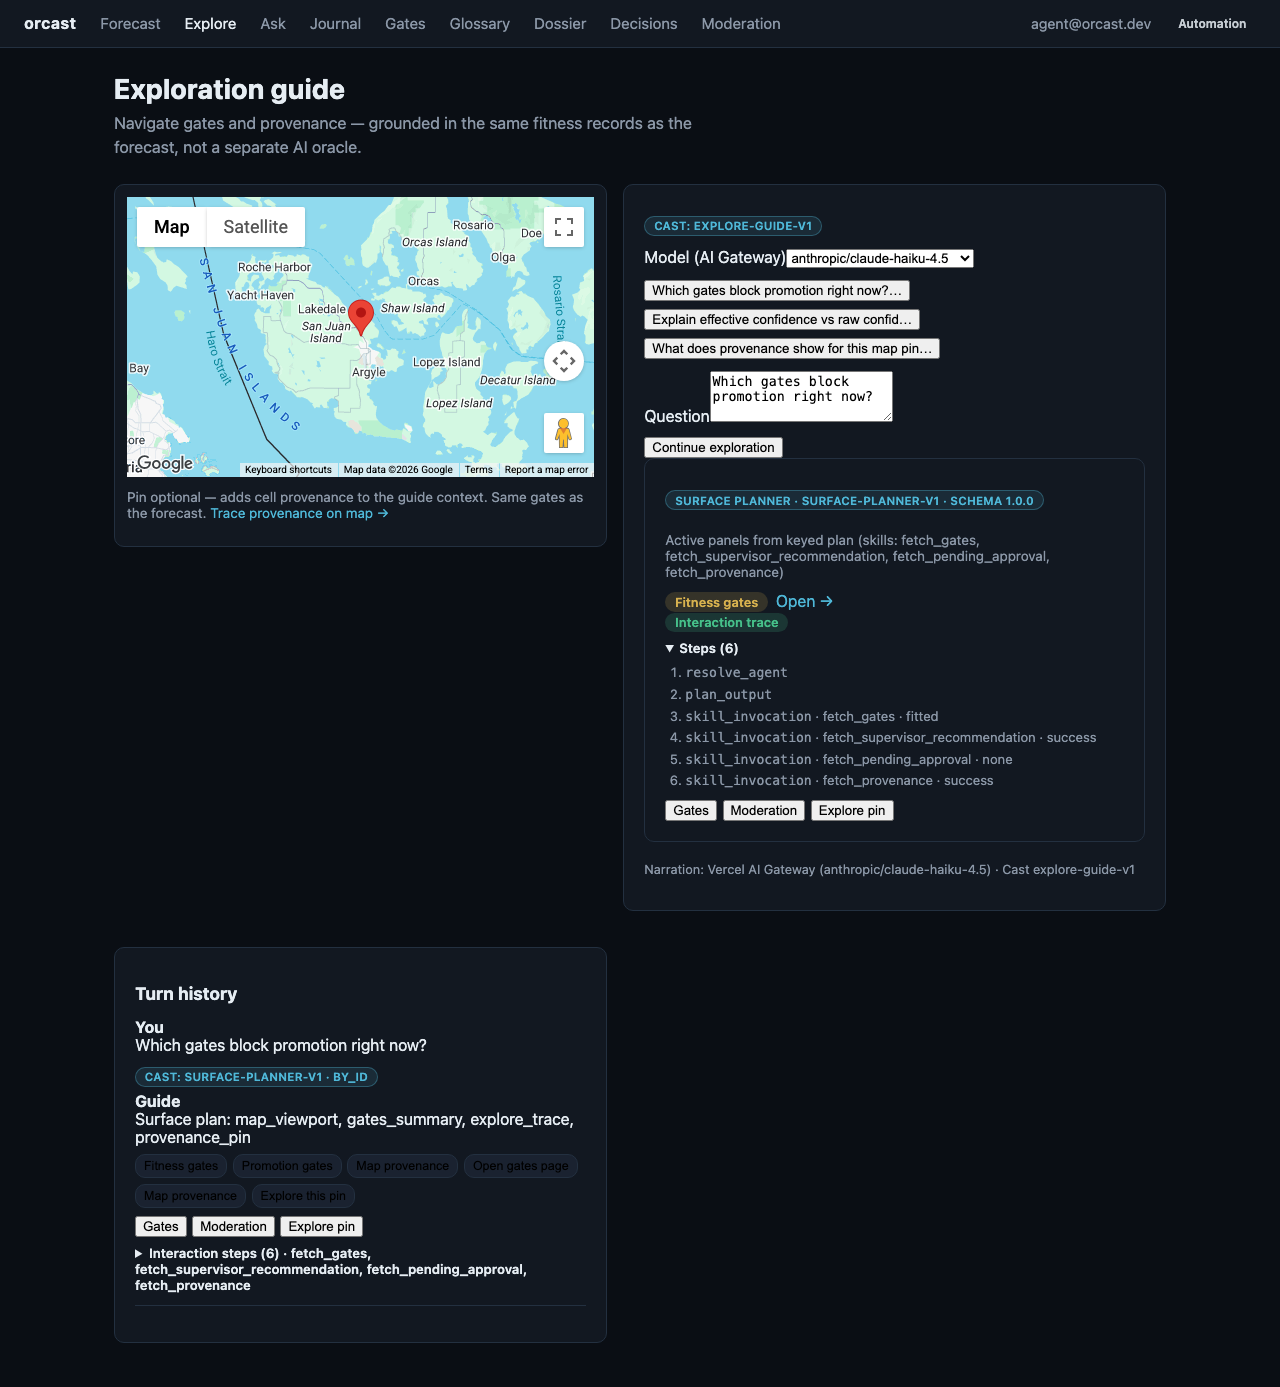
\includegraphics[width=\linewidth]{beat-04-planner.png}
\end{center}

\textbf{Storyboard intent.} Show Central Casting: the managed agent resolves a cast role, dispatches skills, and produces a structured step-log with grounding references before narrating.

\textbf{What a judge sees.} Explore page with a map (small, left column) and a chat panel (right). The cast badge ``CAST: EXPLORE-GUIDE-V1'' is visible. The question ``Which gates block promotion right now?'' is pre-filled. The response shows ``SURFACE PLANNER $\cdot$ SURFACE-PLANNER-V1 $\cdot$ SCHEMA 1.0.0'' with a 6-step interaction trace expanded: resolve\_agent, plan\_output, 4 skill\_invocations. Deep-link buttons: Gates, Moderation, Explore pin. Narration credit: Vercel AI Gateway.

\textbf{What is missing or confusing.}
\begin{itemize}
\item The cast badge says ``EXPLORE-GUIDE-V1'' (the chat agent) but the panel header shows ``SURFACE PLANNER $\cdot$ SURFACE-PLANNER-V1''. The distinction between the explore guide and the surface planner is not clear to a judge.
\item The 6-step trace is collapsed in a disclosure widget. A judge watching video will not expand it in the 15 seconds this beat is on screen.
\item The grounding benchmark claim (0\% uncited rate) belongs here but Beat 4b was excluded from the recording. The benchmark is the strongest proof-point and it does not appear on camera.
\end{itemize}

\begin{p1box}
\textbf{P1, Consider re-including Beat 4b.} The grounding benchmark (0\% uncited) is the strongest AMI-alignment proof point. A 15-second static slide showing the figure-mp3 benchmark scope diagram would add it. The demo is 2m 12s, 15 more seconds is acceptable.
\end{p1box}

% ─────────────────────────────────────────────────────────────────────────────
\subsection{Beat 05, Sighting check (\texttt{/ask})}

\begin{center}
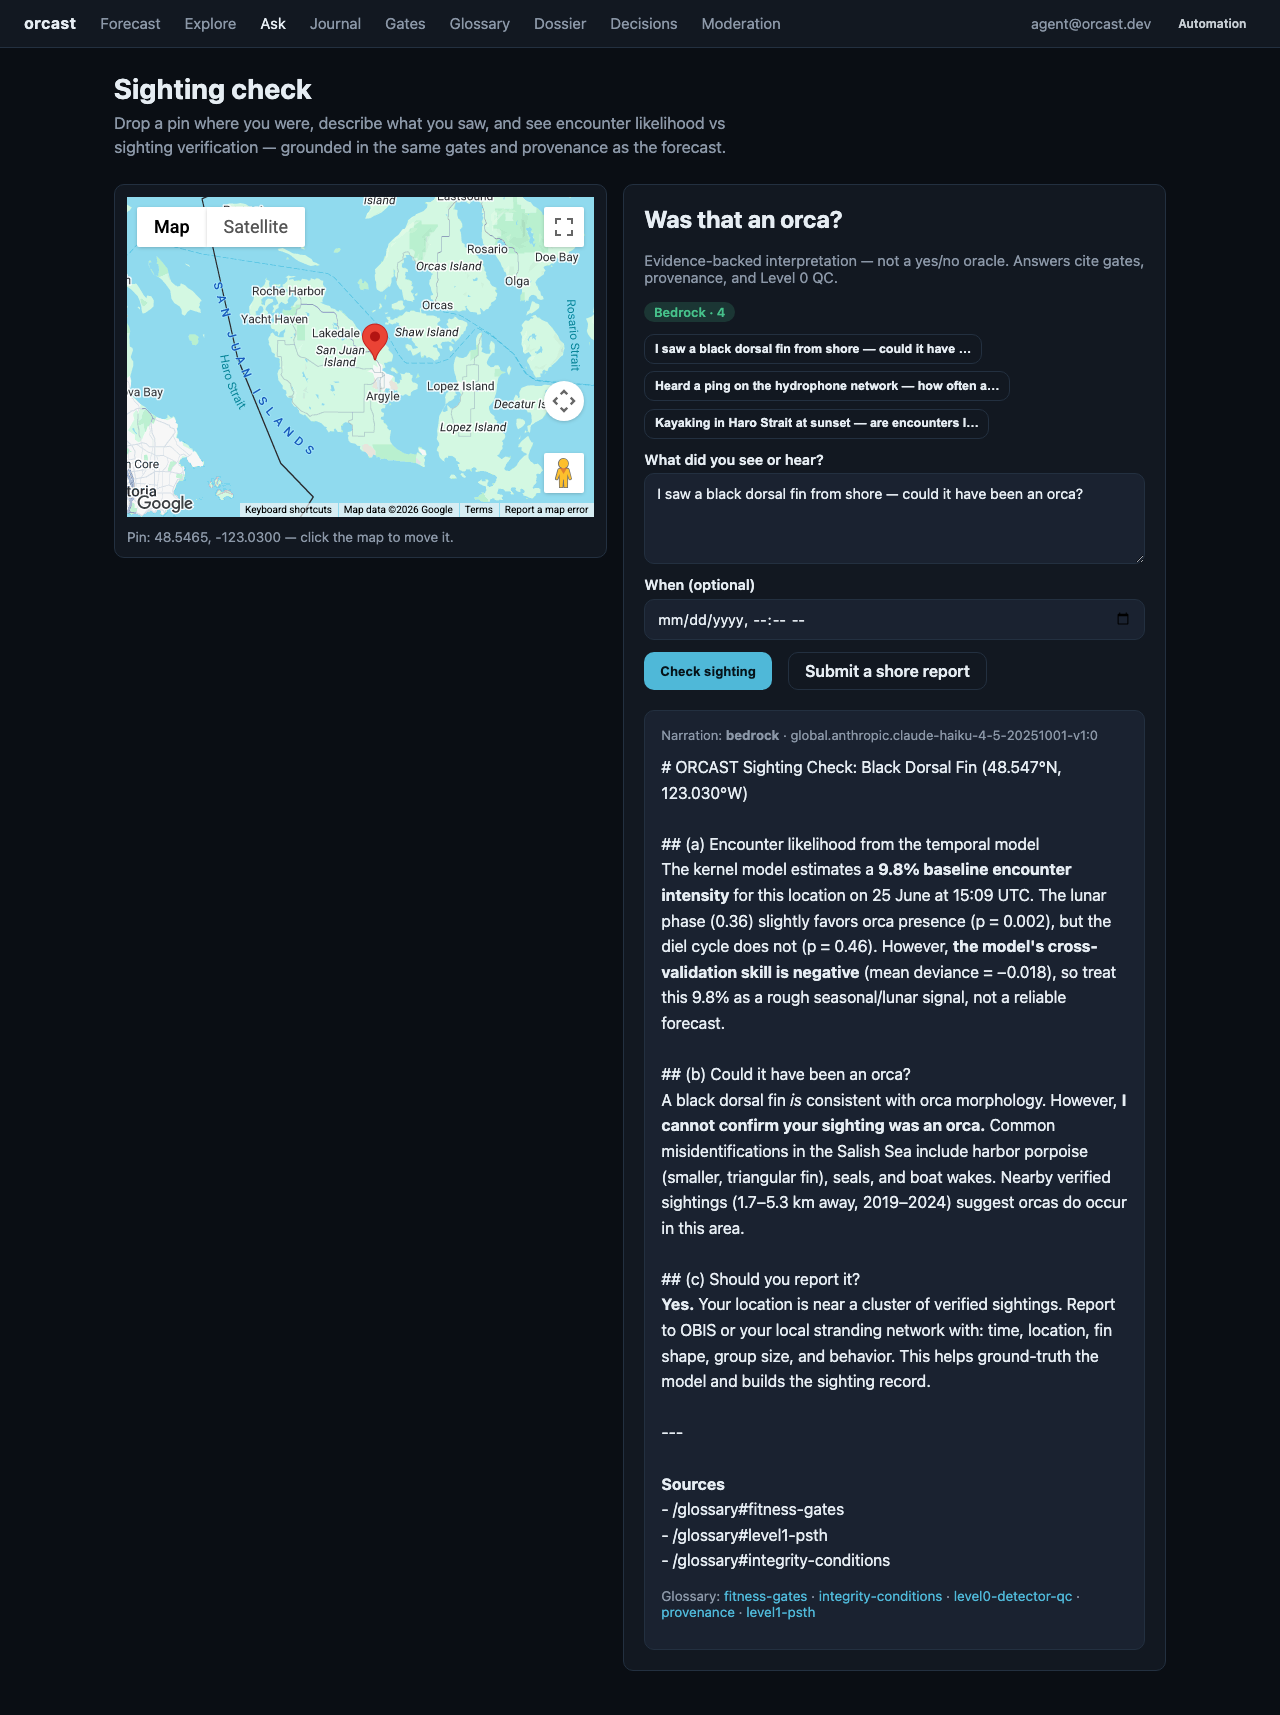
\includegraphics[width=\linewidth]{beat-05-ask.png}
\end{center}

\textbf{Storyboard intent.} Show that the sighting check separates encounter likelihood from species identification, grounded in the gate data, not a yes/no oracle.

\textbf{What a judge sees.} A structured 3-part Bedrock response: (a) encounter likelihood 9.8\% baseline, lunar favours presence, but cross-validation skill is negative so treat cautiously; (b) cannot confirm the sighting was an orca; (c) yes, report it with instructions and nearby verified sightings context. Sources linked at bottom. Bedrock badge visible.

\textbf{What is missing or confusing.}
\begin{itemize}
\item The pre-filled question ``I saw a black dorsal fin from shore, could it have been an orca?'' makes it obvious this is a seeded demo rather than a live sighting check.
\item The ``Submit a shore report'' button is visible but the flow from sighting check to journal to moderation is not demonstrated in this beat, it requires context from Beat 06.
\end{itemize}

\begin{notebox}
\textbf{No P0 or P1 gaps.} This is the strongest beat. The response quality is high, the limits are disclosed honestly, and the Bedrock attribution is visible. The main note is that the pre-filled question is obviously seeded, acceptable for a Playwright demo.
\end{notebox}

% ─────────────────────────────────────────────────────────────────────────────
\subsection{Beat 06a, Field journal (\texttt{/journal})}

\begin{center}
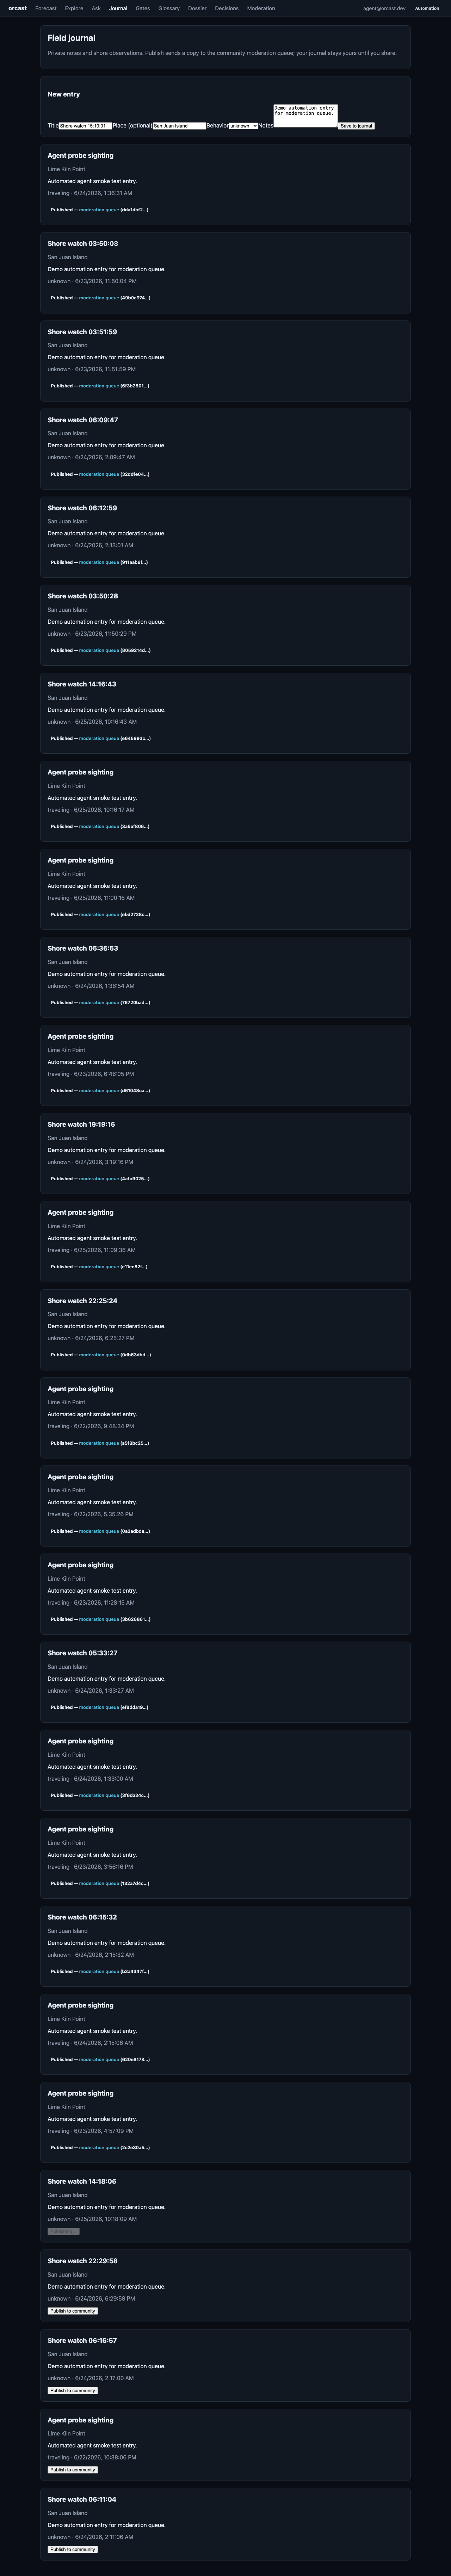
\includegraphics[width=\linewidth]{beat-06-journal.png}
\end{center}

\textbf{Storyboard intent.} Show that field notes are private until the observer publishes them to the community queue.

\textbf{What a judge sees.} A long list of journal entries, all reading ``agent orcast sighting $\cdot$ Lime Kiln Point $\cdot$ agent@orcast.dev $\cdot$ Automated agent smoke test entry.'' Multiple identical entries, same location, same content, same observer.

\begin{p0box}
\textbf{P0, The journal is full of automated smoke test entries.} This is the most damaging beat in the deck. A judge sees what looks like a system filling its own journal with junk data, not field researchers posting notes. The ``Automated agent smoke test entry.'' label and the dozens of identical entries make it obvious this is test scaffolding.

\textbf{Fix before Saturday.} Option A (preferred): Before re-recording, manually create 3--5 realistic journal entries from the test user (e.g.\ ``Transiting pod, 5+ animals, foraging behaviour near Shaw Island'') and delete the smoke test entries. Option B: Seed realistic entries via the agent credentials during the Playwright setup step rather than using the generic smoke test content. The journal beat must show what a field researcher would actually write.
\end{p0box}

% ─────────────────────────────────────────────────────────────────────────────
\subsection{Beat 06b, Community moderation queue (\texttt{/moderation})}

\begin{center}
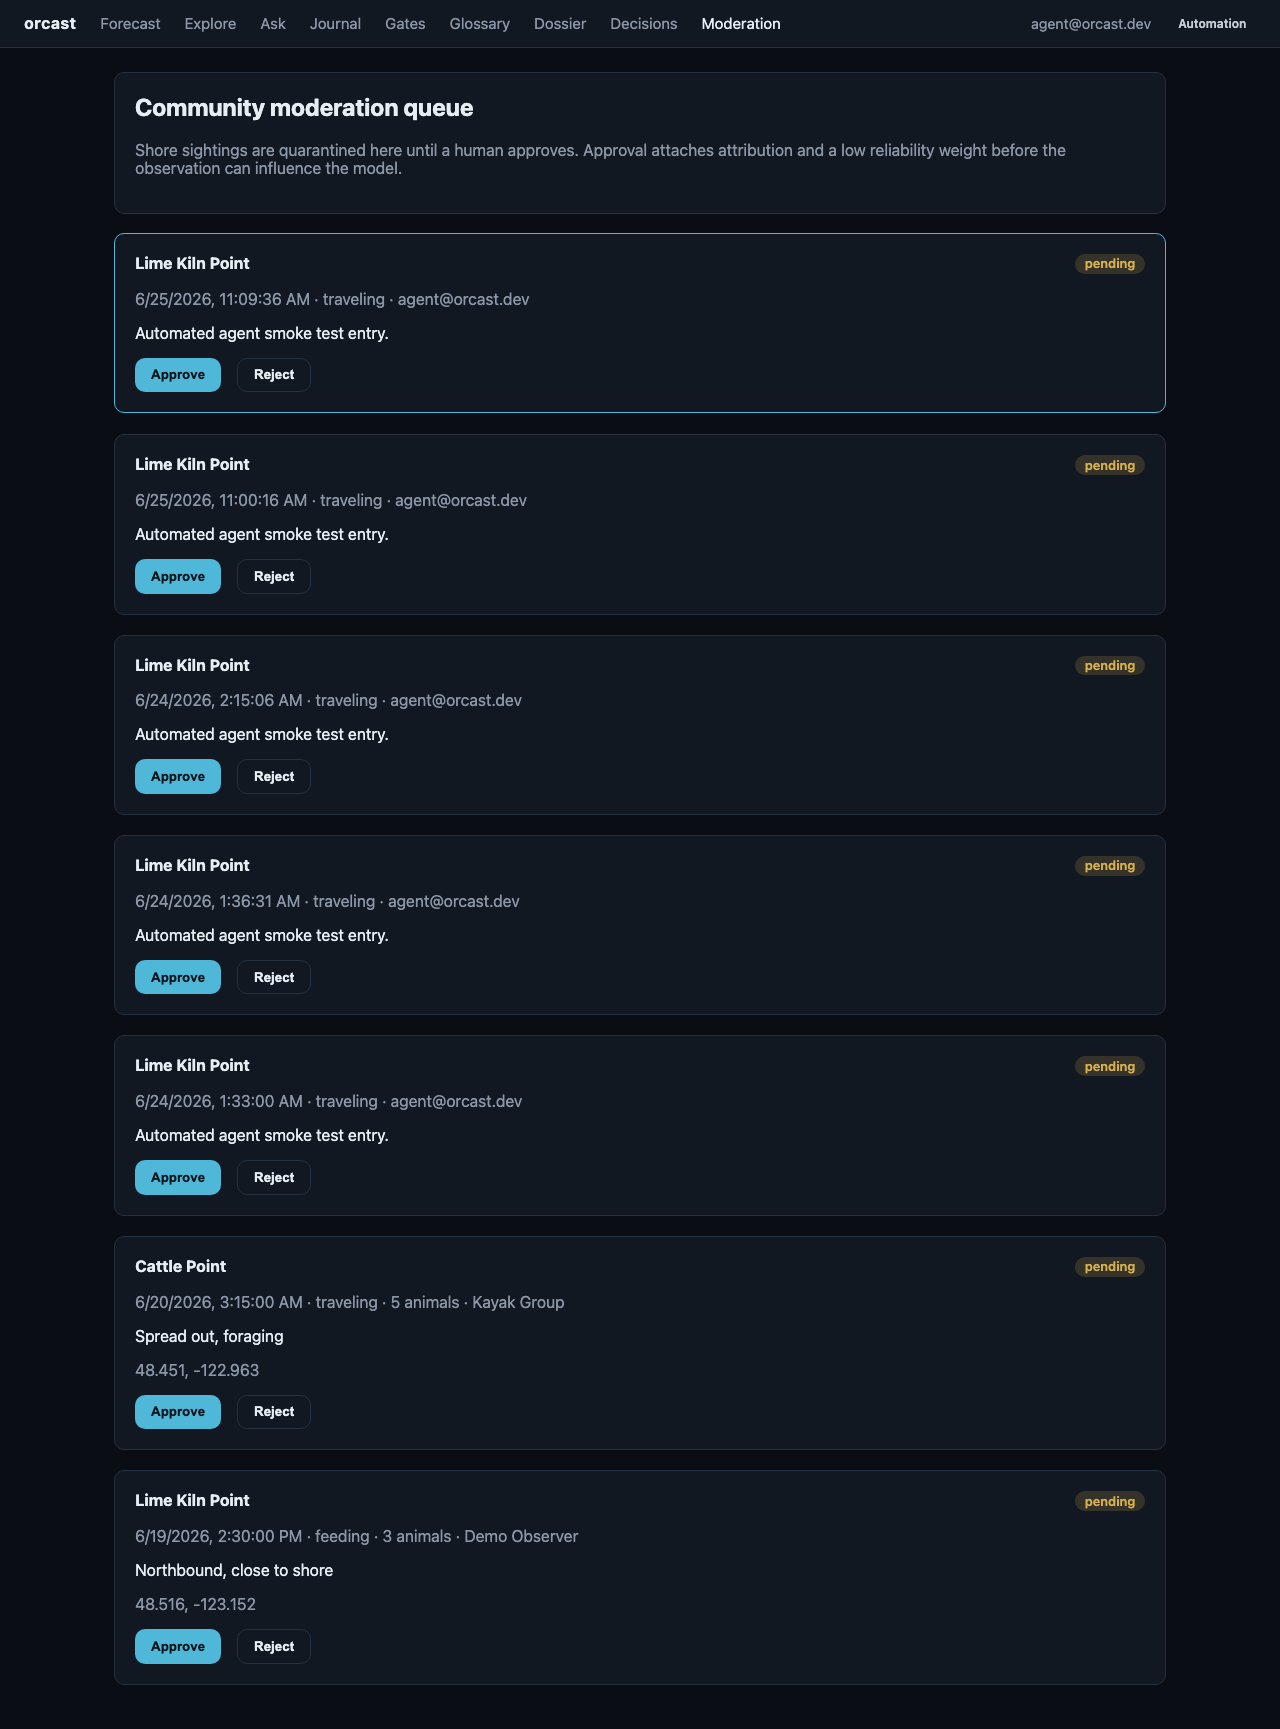
\includegraphics[width=\linewidth]{beat-06-moderation.png}
\end{center}

\textbf{Storyboard intent.} Show that shore reports are quarantined until a human approves. Approval attaches attribution and a low reliability weight before the observation influences the model.

\textbf{What a judge sees.} Community moderation queue with 7+ pending entries. The first 5 are ``Lime Kiln Point $\cdot$ Automated agent smoke test entry.'' from agent@orcast.dev. The bottom two are real-looking: ``Cattle Point $\cdot$ Spread out, foraging $\cdot$ 5 animals $\cdot$ Kayak Group'' and ``Lime Kiln Point $\cdot$ Northbound, close to shore $\cdot$ 3 animals $\cdot$ Demo Observer''.

\textbf{What is missing or confusing.}
\begin{itemize}
\item The 5 smoke test entries at the top of the queue contradict the citizen-science framing.
\item The real sightings at the bottom are good but buried under test data.
\end{itemize}

\begin{p1box}
\textbf{P1, Clear smoke test entries from the queue before re-recording.} Approve or reject the smoke test entries so only realistic submissions appear. The queue then shows what the governance workflow is actually for: real field data being reviewed before it influences the model.
\end{p1box}

% ─────────────────────────────────────────────────────────────────────────────
\subsection{Beat 07, DynamoDB proof slide}

\begin{center}
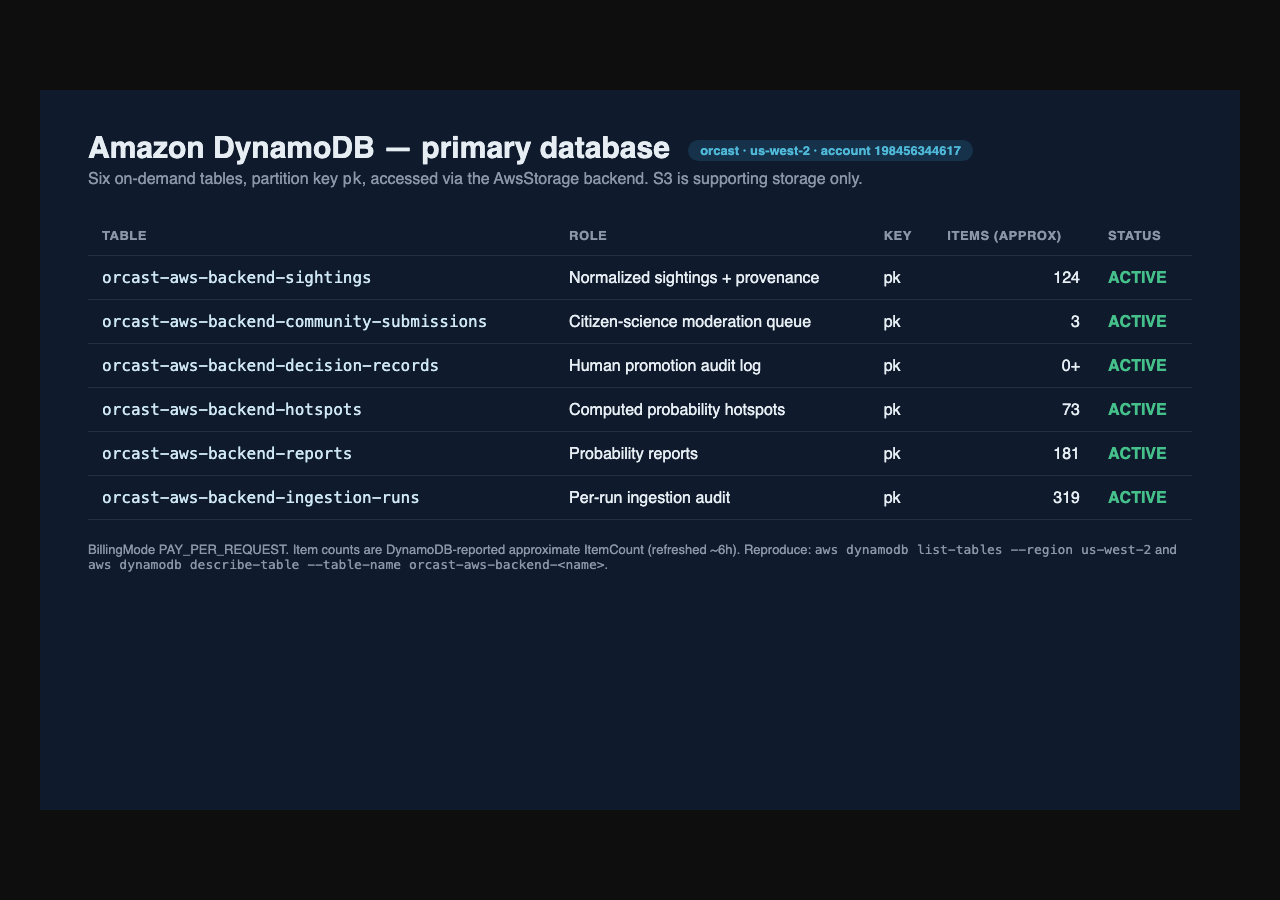
\includegraphics[width=\linewidth]{beat-07-dynamodb.png}
\end{center}

\textbf{Storyboard intent.} Show that DynamoDB is the primary system of record with all nine on-demand tables active.

\textbf{What a judge sees.} A static slide titled ``Amazon DynamoDB -- primary database'' with a table listing 6 entries. Subtitle: ``Six on-demand tables.'' Tables shown: sightings (124), community-submissions (3), decision-records (0+), hotspots (73), reports (181), ingestion-runs (319).

\begin{p0box}
\textbf{P0, The slide shows 6 tables and says ``Six on-demand tables.'' The submission claims 9 tables.} The missing tables are: user-journal, partner-api-keys, managed-agents. The subtitle and table count directly contradict the submission copy and the whitepaper.

Additionally, \texttt{decision-records} shows ``0+'' items. The live database has 3 items (confirmed by Q1c). This is a DynamoDB approximate ItemCount cache lag but it reads as ``zero records'' to a judge.

\textbf{Fix before Saturday.} Update \texttt{web/public/demo-slides/dynamodb-proof.png} to show all 9 tables. Options: (a) update the static HTML/image that generates the proof slide; (b) take a fresh AWS Console screenshot showing all 9 tables; (c) rebuild the slide with the correct table list and live item counts. Priority: this is the only piece of direct database evidence in the submission, it must show 9 tables.
\end{p0box}

% ─────────────────────────────────────────────────────────────────────────────
\subsection{Beat 08, Architecture close (static slide)}

\begin{center}
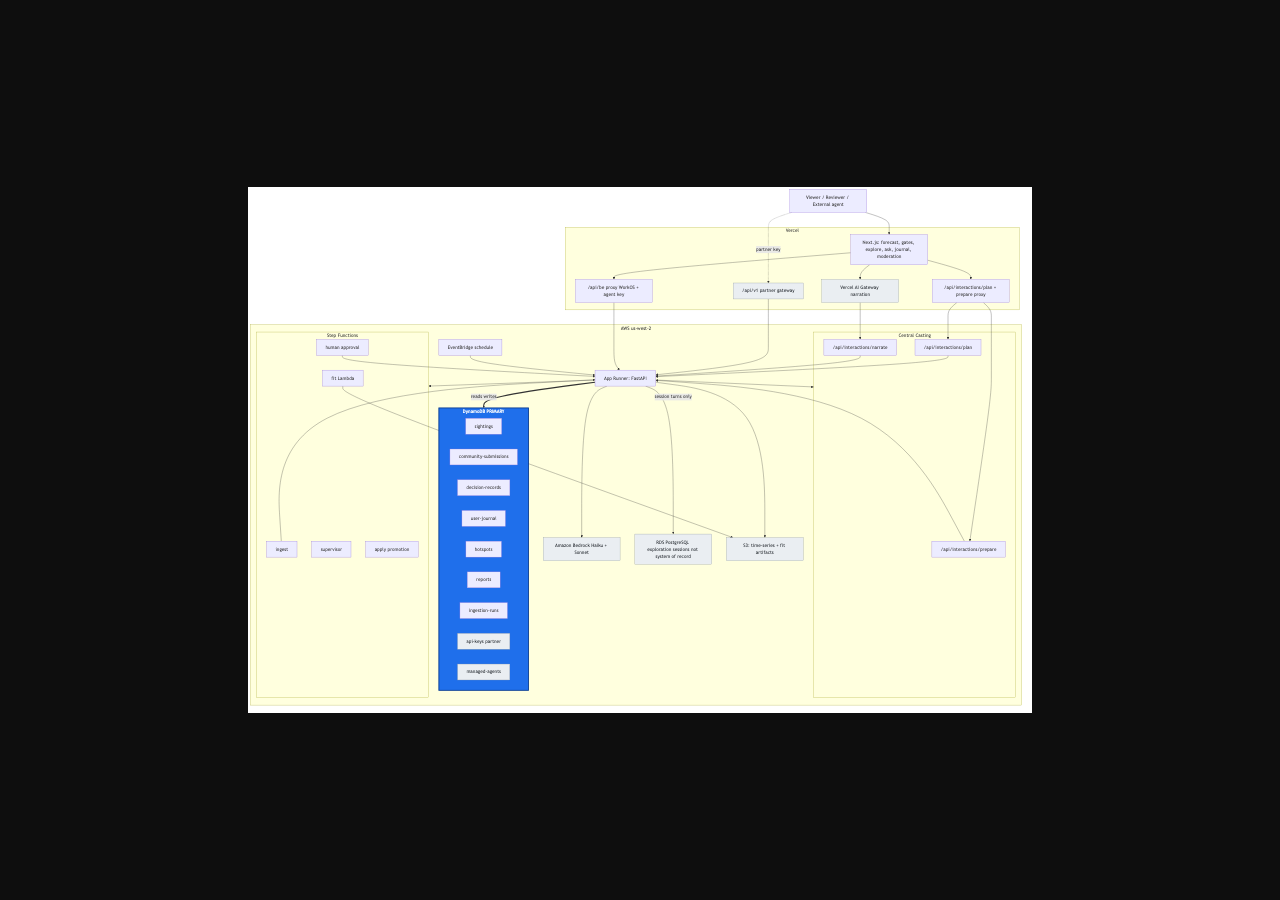
\includegraphics[width=\linewidth]{beat-08-architecture.png}
\end{center}

\textbf{Storyboard intent.} Close the demo with the full system architecture diagram showing all deployed services.

\textbf{What a judge sees.} A white diagram with a light yellow auto-layout box structure. The Mermaid-generated architecture diagram, the OLD version with the DynamoDB column of boxes in the centre. The new TikZ fig-08 architecture diagram (four-band, clean, corrected Vercel AI Gateway label) was built but is not what appears here.

\begin{p0box}
\textbf{P0, Beat 08 shows the old Mermaid architecture diagram, not the new TikZ fig-08.} The new TikZ diagram was built and copied to \texttt{web/public/demo-slides/architecture.png} in the Q2 remediation. But this beat screenshot shows the old Mermaid version. Either the copy did not take effect, or the Playwright screenshot was captured before the file was replaced.

\textbf{Fix before re-recording.} Verify that \texttt{web/public/demo-slides/architecture.png} is the new TikZ figure (check file size and timestamp), then re-run the demo recording. The new diagram has a five-band layout with correct Vercel AI Gateway labelling, DynamoDB as primary system of record, and Central Casting properly boxed.
\end{p0box}

\newpage
\section{Section 2: Submission Copy Audit}

The DEVPOST\_DRAFT claims are reproduced below, each annotated with: (a) the live evidence that backs it, and (b) a flag if the claim is harder to demonstrate than it reads.

\subsection{Project title and tagline}

\begin{notebox}
\textbf{Title:} Physical world model fusion for orca encounter forecasting and community platform for field researchers\\
\textbf{Tagline:} Every map cell's confidence is bounded by a statistical gate battery. Every agent action is logged and citable. Every community sighting is quarantined until a human signs off.
\end{notebox}

\textbf{Review.} The tagline makes three claims. All three are true:
\begin{enumerate}
\item Gate battery bounds confidence $\to$ demonstrated in Beat 03 (gates page) and confirmed by effective\_confidence in the API.
\item Agent actions logged and citable $\to$ demonstrated in Beat 04 (step-log expanded in interaction trace). \Ppp{The step-log requires clicking the disclosure widget, it is not immediately visible.}
\item Community sighting quarantined until human signs off $\to$ demonstrated in Beat 06b (moderation queue). \Pp{The queue is full of smoke test entries in the current recording.}
\end{enumerate}

\subsection{Feature bullets}

\textbf{Always-on forecast with inline confidence governed by fitness gates + human promotion.}
\begin{notebox}
\OK{} Beat 01 shows the forecast always on. Beat 03 shows the gates. The 0\% confidence is accurate. \Pp{A judge might interpret 0\% as ``the system is not working.'' The narration must explain why 0\% is the correct honest answer.}
\end{notebox}

\textbf{Click-to-trace provenance: kernels, gate verdicts, nearby evidence per map cell.}
\begin{notebox}
\OK{} Beat 02 shows the provenance modal with kernels and integrity conditions. \Po{} The PSTH kernel plots render as blank white boxes (offline fit artifact). This must be fixed before the demo is re-recorded or the screenshot submitted.
\end{notebox}

\textbf{Gates dashboard with integrity conditions and Level 1 PSTH visuals + glossary.}
\begin{notebox}
\OK{} Beat 03 shows the full gates page. \Po{} PSTH visuals are blank white boxes. Level 1 PSTH section of the claim is not demonstrated in the current recording.
\end{notebox}

\textbf{Sighting check: Bedrock-grounded chat separating encounter likelihood from species identification.}
\begin{notebox}
\OK{} Beat 05 is the strongest beat. Response is high quality, limits are disclosed, Bedrock attribution is visible. No gap.
\end{notebox}

\textbf{Field journal: private notes; publish sends a copy to the community moderation queue.}
\begin{notebox}
\Po{} Beat 06a shows a journal full of automated smoke test entries. The ``private notes'' framing requires realistic content. The journal beat actively undermines this claim in the current recording.
\end{notebox}

\textbf{Citizen-science moderation: quarantined in DynamoDB until a WorkOS-signed reviewer approves.}
\begin{notebox}
\Pp{} Beat 06b shows the queue but the first 5 entries are smoke test entries. The real sightings at the bottom of the queue make the governance intent visible but not prominent. Clear smoke test entries before re-recording.
\end{notebox}

\textbf{Exploration guide / surface planner via Central Casting.}
\begin{notebox}
\OK{} Beat 04 shows the surface planner with the 6-step interaction trace. The CAST badge, skill invocations, and step-log are all visible. \Ppp{The map is small relative to the chat panel. The explore guide and surface planner are conflated in the cast badge label.}
\end{notebox}

\textbf{Grounding quality benchmark: step-log reduces $R_\text{uncited}$ from 91\% to 0\%.}
\begin{notebox}
\Pp{} This claim is in the Devpost description but does not appear on camera in the current recording (Beat 4b was excluded). This is the strongest AMI-alignment proof point. Consider re-including the 15-second benchmark slide as Beat 4b.
\end{notebox}

\textbf{Immutable promotion audit log.}
\begin{notebox}
\Ppp{} Not shown on camera. The decision-records DynamoDB table exists (3 items confirmed by Q1c) but no beat shows it directly. The DynamoDB proof slide (Beat 07) should include decision-records with a non-zero count.
\end{notebox}

\subsection{DynamoDB section}

\begin{notebox}
The submission copy says: ``Nine on-demand tables in us-west-2: \texttt{sightings}, \texttt{community-submissions}, \texttt{decision-records}, \texttt{user-journal}, \texttt{hotspots}, \texttt{reports}, \texttt{ingestion-runs}, \texttt{partner-api-keys}, \texttt{managed-agents}.''
\end{notebox}

\begin{p0box}
\textbf{P0, The DynamoDB proof slide (Beat 07) shows 6 tables and says ``Six on-demand tables.''} This directly contradicts the submission copy. The three missing tables (user-journal, partner-api-keys, managed-agents) are not shown. Fix: rebuild the dynamodb-proof.png slide with all 9 tables before the next recording.
\end{p0box}

\subsection{Screenshot proving AWS Database usage}

\begin{notebox}
The submission says: ``AWS Console screenshot showing nine \texttt{orcast-aws-backend-*} tables.''
\end{notebox}

\begin{p0box}
\textbf{P0, No such screenshot exists in the submission materials.} The fallback is \texttt{docs/devpost/figures/dynamodb-proof.png} which shows only 6 tables. Take an actual AWS Console screenshot of the DynamoDB Tables view showing all 9 tables before submitting.
\end{p0box}

\subsection{Checklist status}

\begin{center}
\begin{tabular}{lll}
\toprule
Item & Status & Note \\
\midrule
Live URL & \textcolor{okgreen}{\textbf{DONE}} & Returns 200 in 1.0s \\
Description & \textcolor{okgreen}{\textbf{DONE}} & Ready to paste \\
Demo video & \textcolor{P1amber}{\textbf{NEEDS RE-RECORD}} & Journal and DynamoDB beats must be fixed first \\
AWS Database & \textcolor{okgreen}{\textbf{DONE}} & DynamoDB confirmed \\
Vercel Team ID & \textcolor{okgreen}{\textbf{DONE}} & team\_dQQph8zC78tTPHDnGnvawdKo \\
Architecture diagram & \textcolor{P0red}{\textbf{VERIFY}} & Confirm new TikZ version is in demo-slides \\
DynamoDB screenshot & \textcolor{P0red}{\textbf{MISSING}} & Take AWS Console screenshot showing 9 tables \\
\bottomrule
\end{tabular}
\end{center}

\newpage
\section{Section 3: Submission Figures Audit}

\subsection{System architecture (fig-08)}

\begin{center}
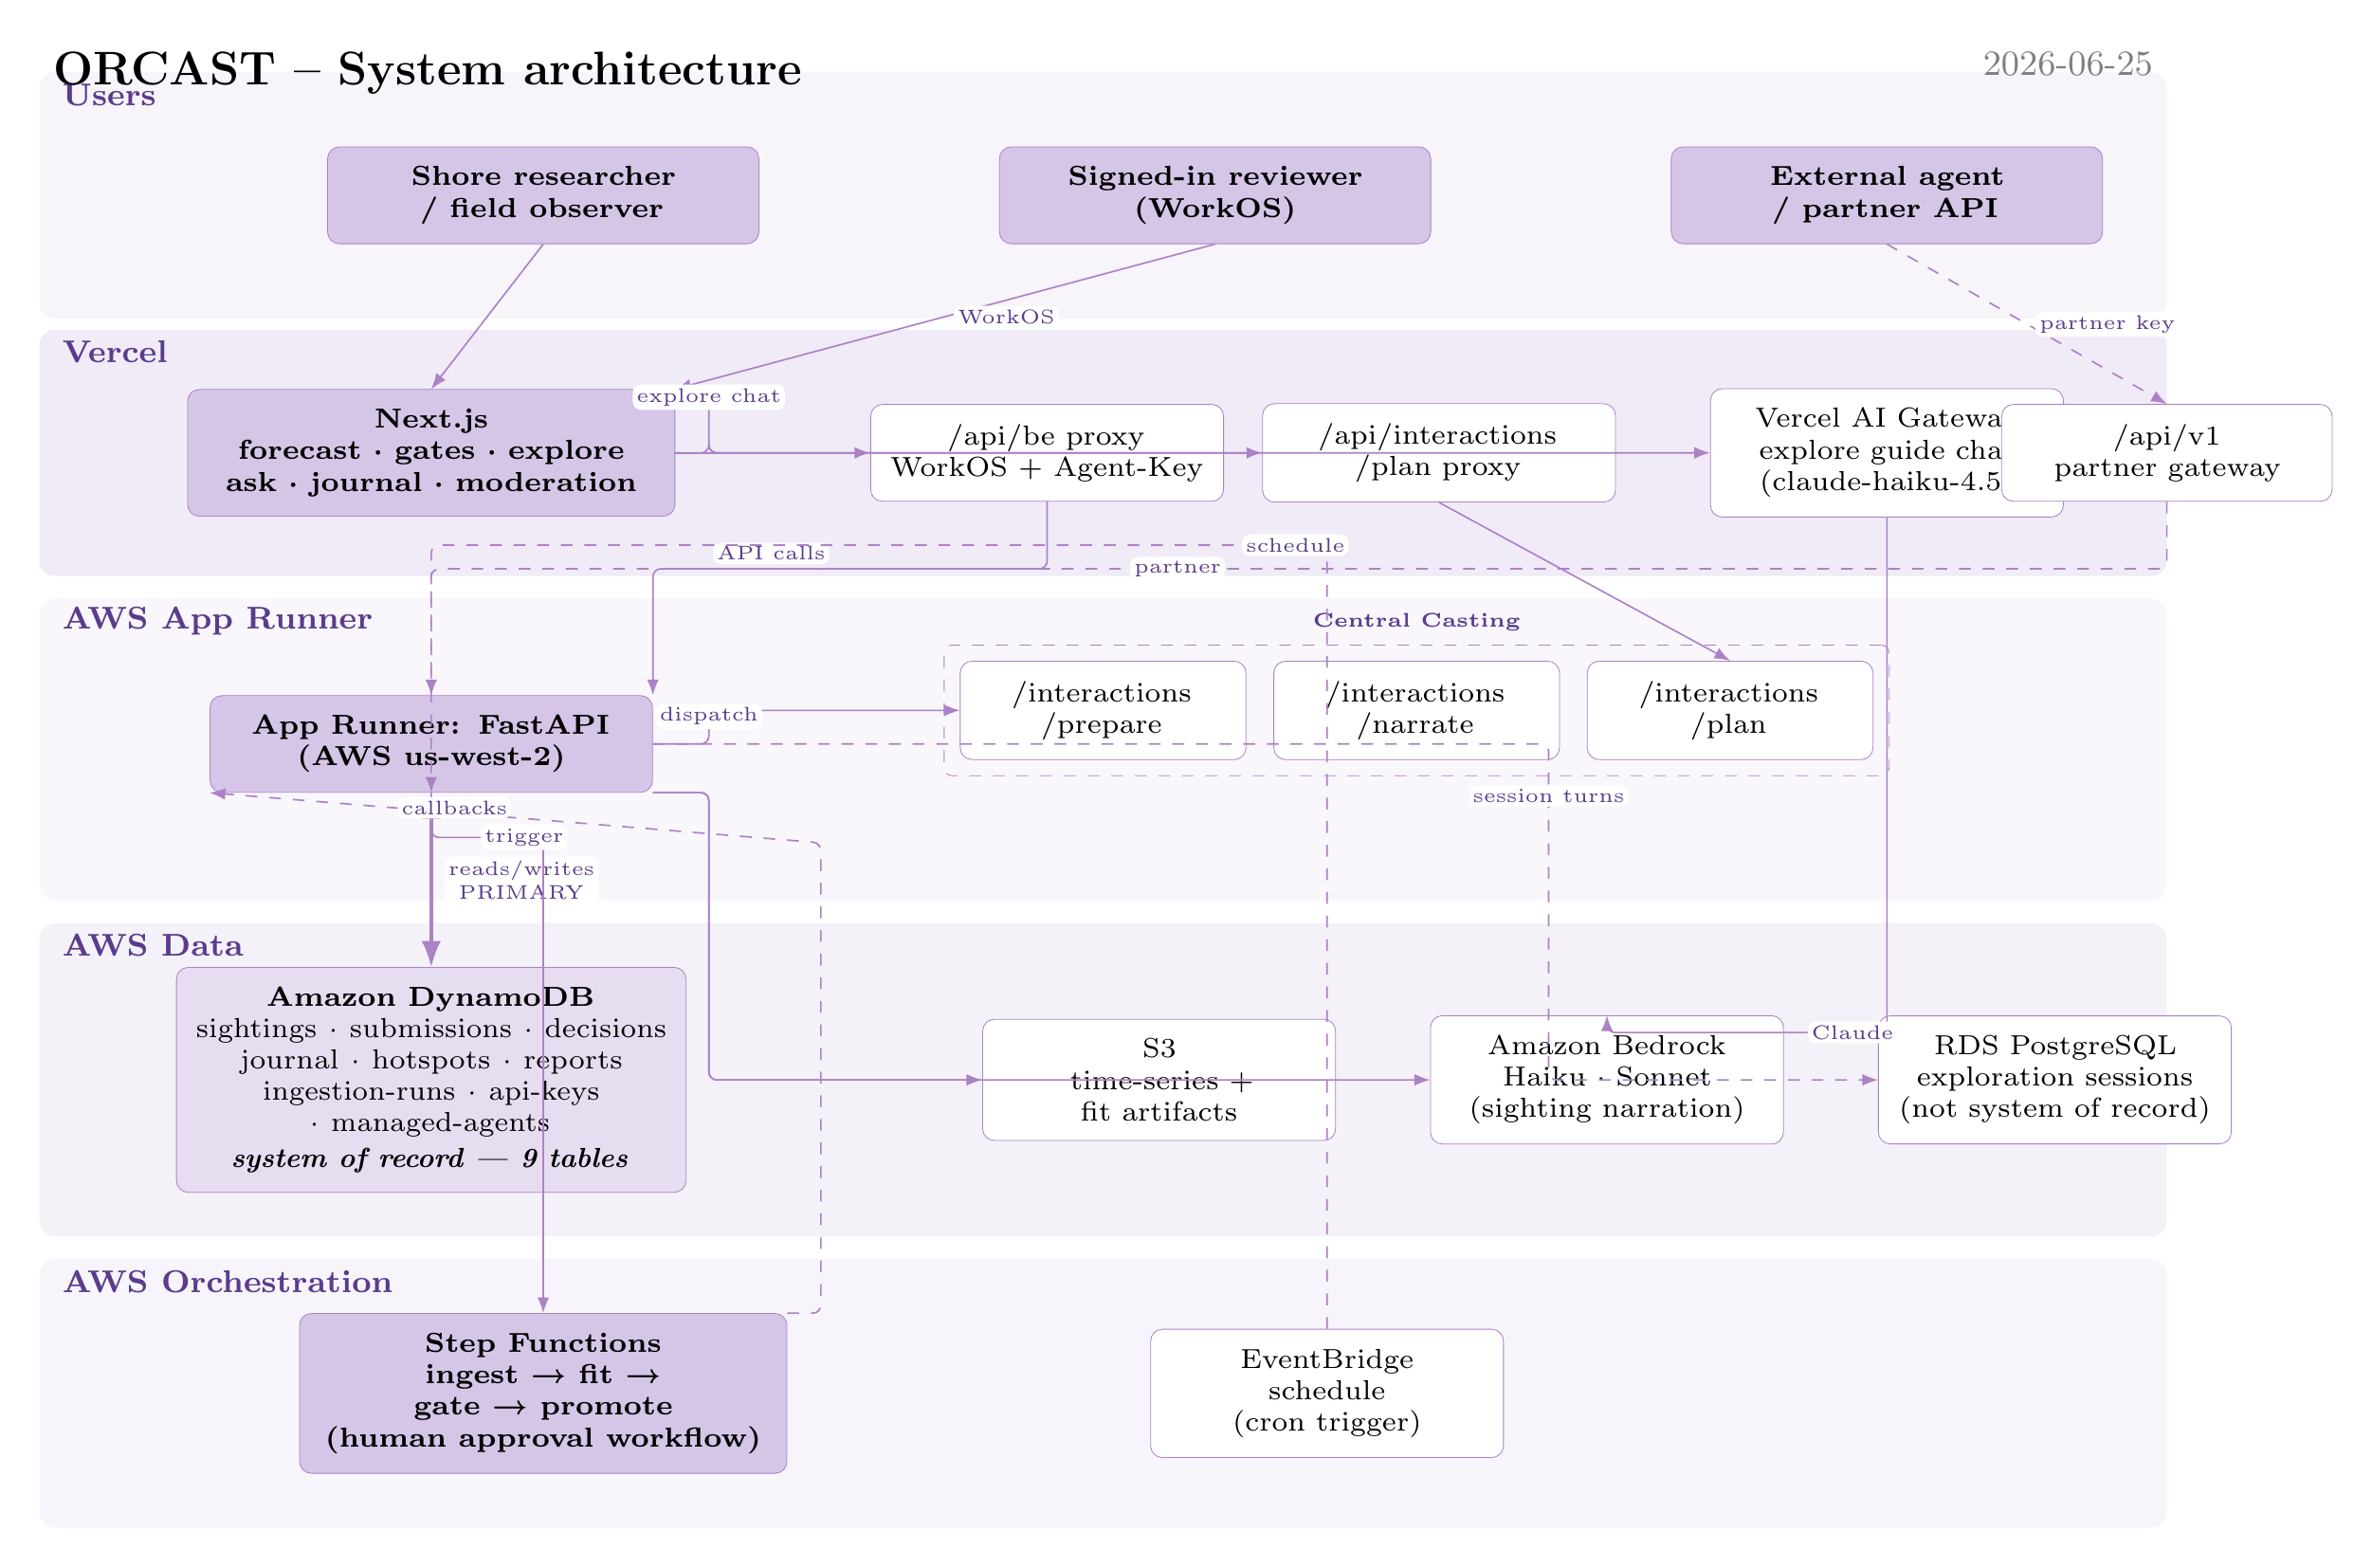
\includegraphics[width=\linewidth]{fig-08-architecture.png}
\end{center}

\textbf{Review.} This is the new TikZ five-band architecture diagram. Compare this with what appears in Beat 08, if Beat 08 shows the old Mermaid auto-layout, the \texttt{web/public/demo-slides/architecture.png} file has not been updated.

\textbf{Adversarial reading.} A judge scanning this in 5 seconds sees: five horizontal bands (Users, Vercel, AWS App Runner, AWS Data, AWS Orchestration), DynamoDB as the central primary box, arrows routing through bands. The Vercel AI Gateway is now correctly labelled as ``explore guide chat (claude-haiku-4.5).''

\textbf{What works.} The band structure communicates the deployment layers clearly. DynamoDB's primacy is visually reinforced. Central Casting is boxed and labelled.

\textbf{What to check before submitting.}
\begin{itemize}
\item The text is small at submission image scale. Check that band labels (``Users'', ``Vercel'', ``AWS App Runner'') are readable when the image is shown at 800px wide.
\item Confirm \texttt{web/public/demo-slides/architecture.png} matches this figure (check file size: should be $\approx$120--140 KB).
\end{itemize}

\begin{p0box}
\textbf{P0, Verify architecture.png in demo-slides is this TikZ version before re-recording.} Run: \texttt{ls -lh web/public/demo-slides/architecture.png}, the file should be $>100$\,KB and dated after June 25. If it is smaller and older, copy the TikZ figure again.
\end{p0box}

% ─────────────────────────────────────────────────────────────────────────────
\subsection{DynamoDB ERD (fig-01)}

\begin{center}
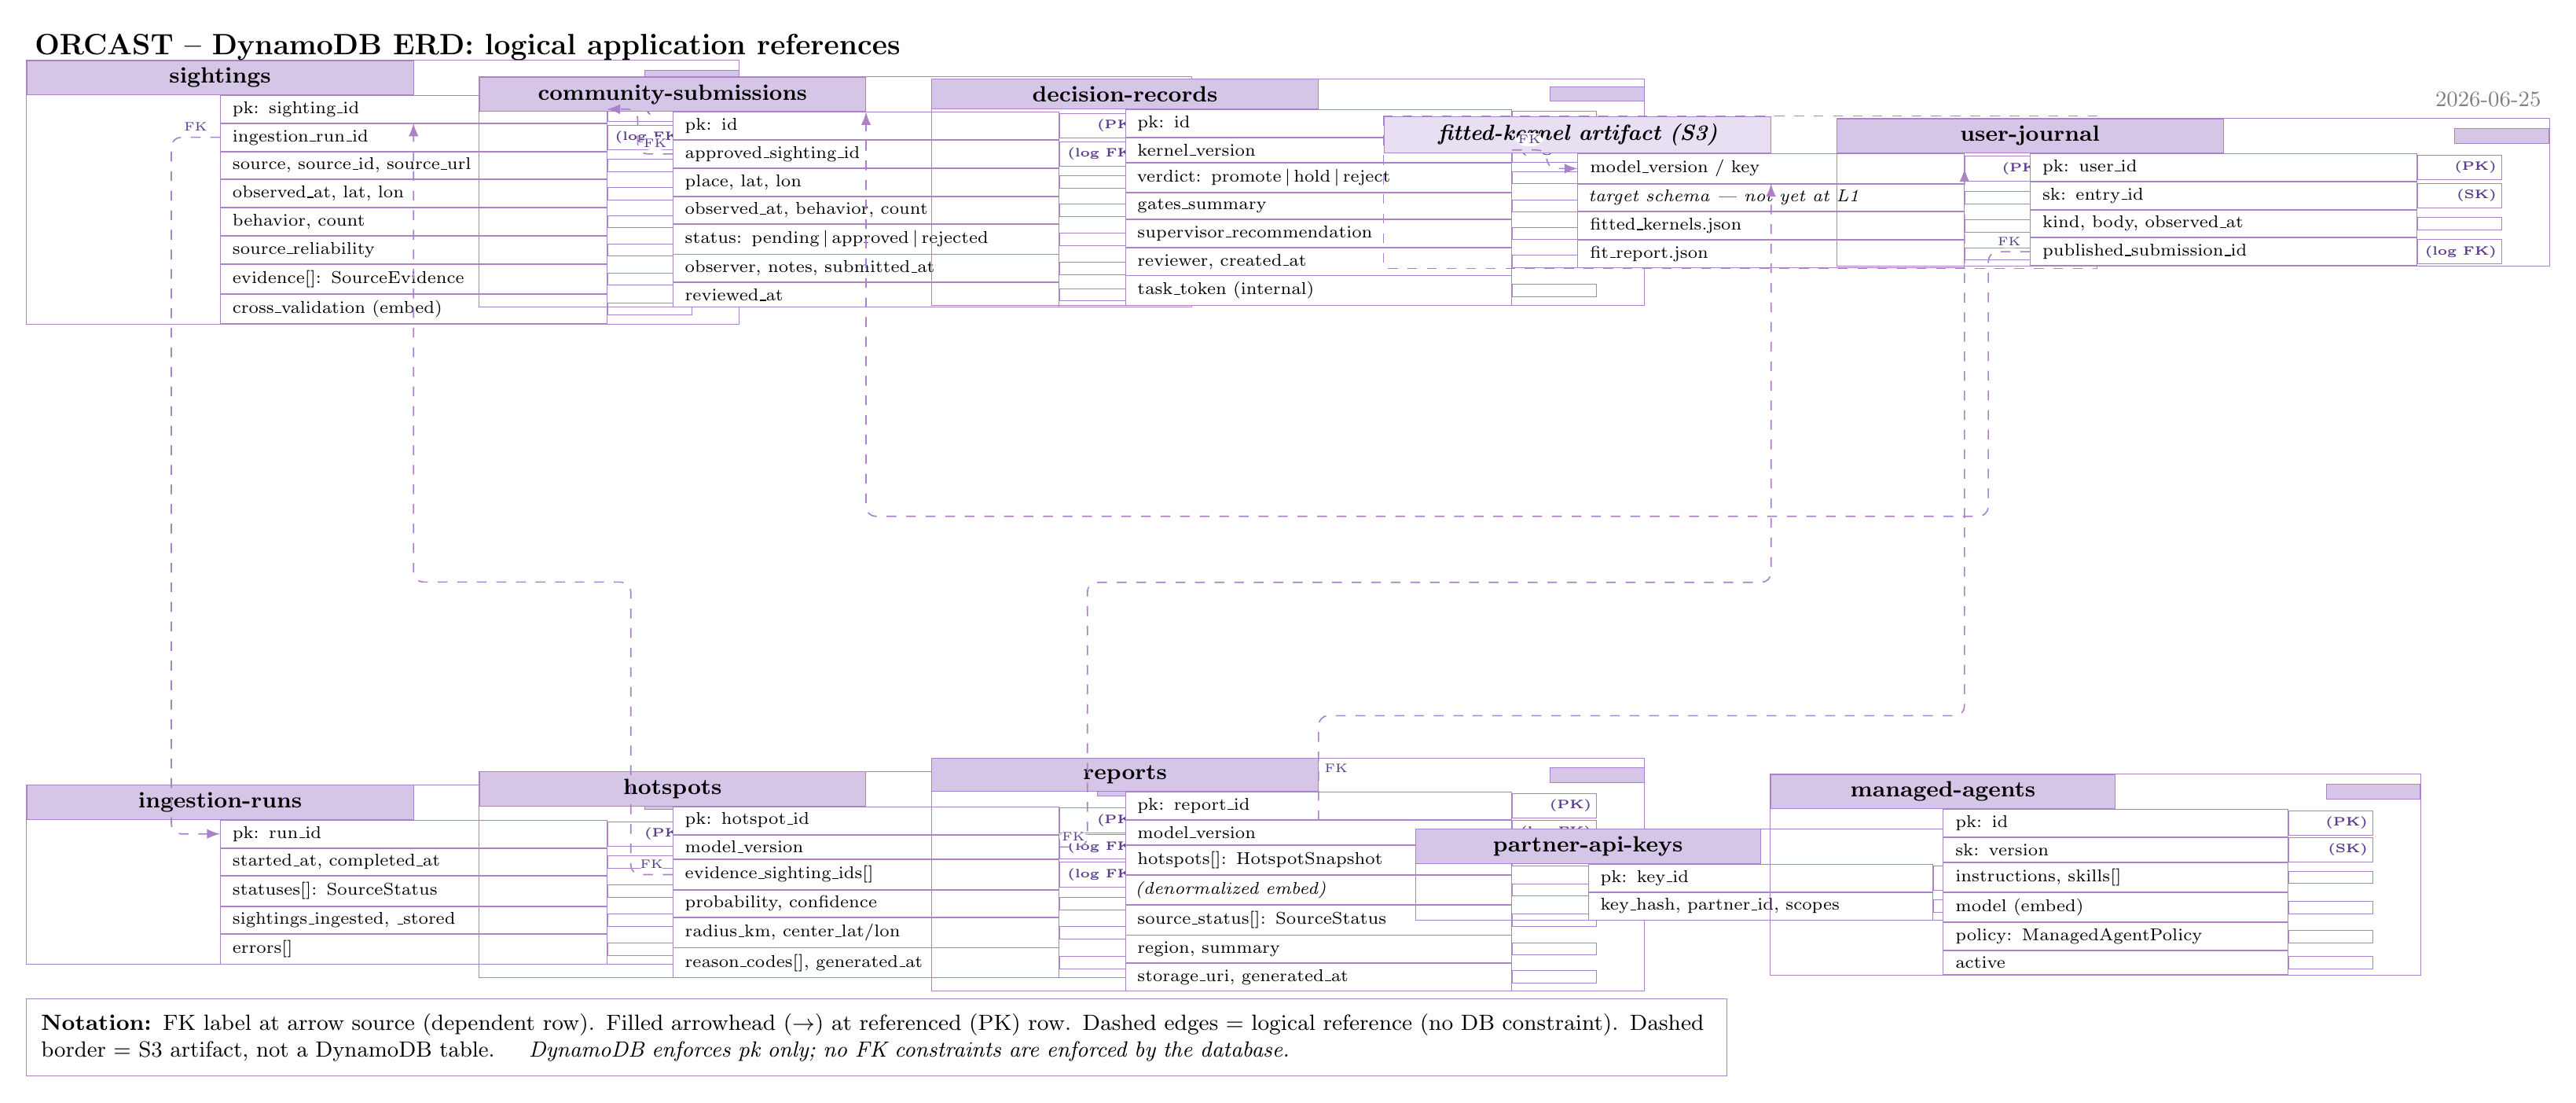
\includegraphics[width=\linewidth]{fig-01-erd.png}
\end{center}

\textbf{Review.} Nine-table ERD with row-level FK edge attachment, lilac headers, and legend. Matches the reference style from the decision-valued maps paper (arXiv:2602.11295, Figure 2).

\textbf{Adversarial reading.} A judge sees clean table boxes and dashed FK arrows. The tables are legible. The ``log FK'' badges on FK rows are accurate (DynamoDB enforces no FK constraints). The notation box at the bottom explains the legend.

\textbf{What works.} Table names are on single lines. Field text does not wrap. FK labels sit at the source (dependent) end. The S3 artifact has a dashed border distinguishing it from DynamoDB tables.

\textbf{Issues.}
\begin{itemize}
\item ``status: pending\,\textbar\,approved\,\textbar\,rejected'' may render as ``status: pending $-$ approved $-$ rejected'' in some rendering environments due to the \texttt{\textbackslash textbar} substitution.
\item At hackathon submission image scale, the field text in the TBLS (small) tables is very small.
\end{itemize}

\begin{notebox}
\textbf{No P0 or P1 gaps.} This figure is publication-quality. Submit as-is.
\end{notebox}

% ─────────────────────────────────────────────────────────────────────────────
\subsection{Grounding benchmark: evidence-binding failure and measurement (fig-mp1)}

\begin{center}
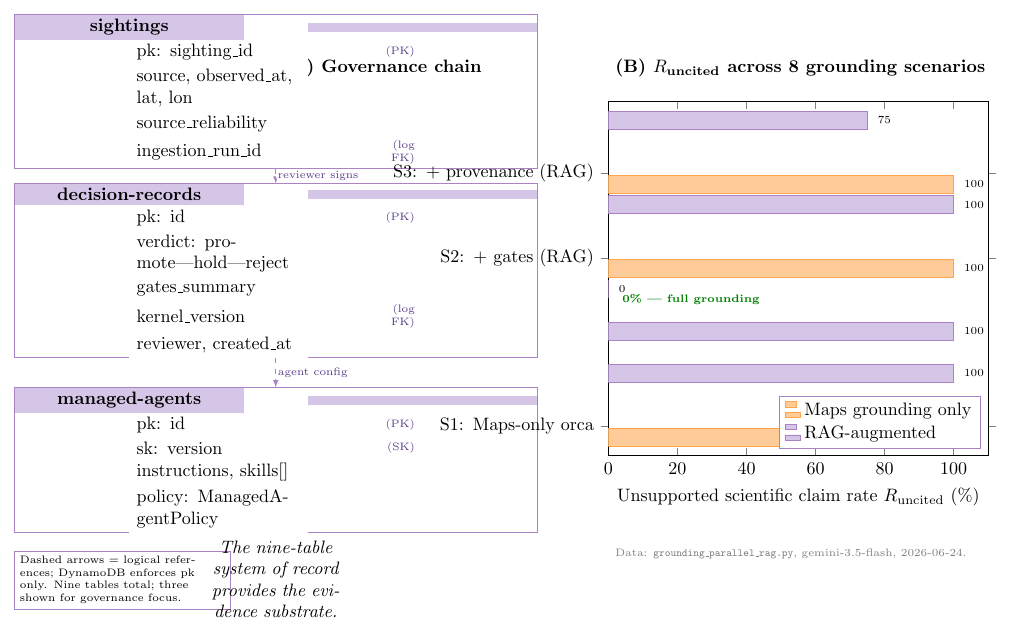
\includegraphics[width=\linewidth]{fig-mp1.png}
\end{center}

\textbf{Review.} Multi-panel Figure 1: (A) orcast governance chain schema, (B) $R_\text{uncited}$ bar chart across 8 scenarios.

\textbf{Adversarial reading.} Panel (A) shows a DynamoDB governance chain diagram, it is a small, dense TikZ figure. Panel (B) shows a bar chart where Scenario 4 (step-log) achieves 0\% and the Maps-only baseline is 60--100\%. The 0\% bar is visually distinct.

\textbf{Issues.}
\begin{itemize}
\item Panel (A) is small and the text inside is very small. A judge may not be able to read the DynamoDB table names.
\item Panel (B) is the critical panel. The ``0\%'' label on the green bar should be readable at submission scale, check this.
\end{itemize}

% ─────────────────────────────────────────────────────────────────────────────
\subsection{Grounding hierarchy and scope (fig-mp3)}

\begin{center}
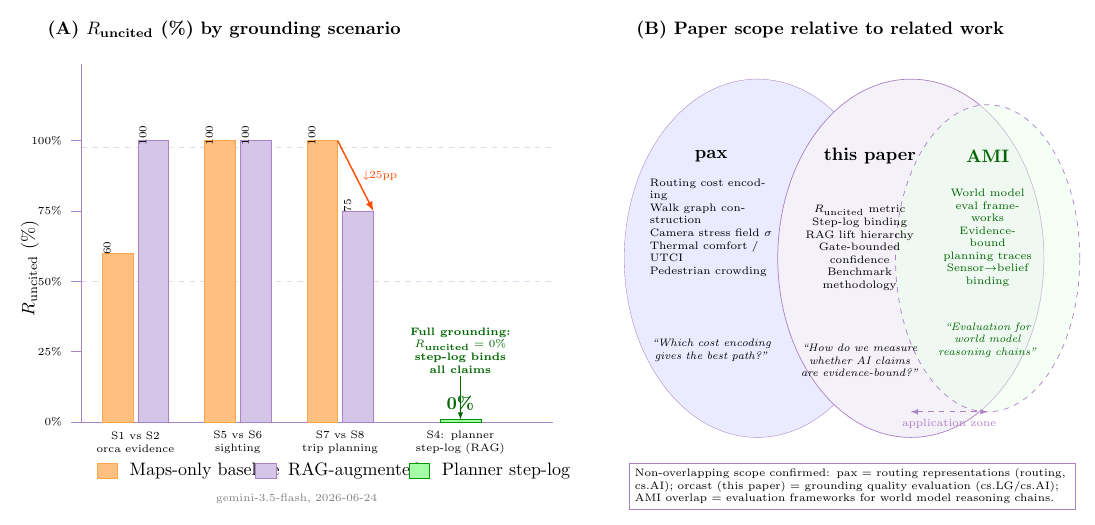
\includegraphics[width=\linewidth]{fig-mp3.png}
\end{center}

\textbf{Review.} Multi-panel Figure 3: (A) $R_\text{uncited}$ hierarchy across scenarios, (B) scope Venn diagram positioning the paper relative to pax and AMI.

\textbf{Adversarial reading.} Panel (A) is the clearest of the three MP figures, a simple bar chart with step-log in green at 0\% and other scenarios in the 60--100\% range. Panel (B) is the scope Venn, three overlapping circles (pax, this paper, AMI). This reads as positioning not evidence.

\textbf{Issues.}
\begin{itemize}
\item Panel (B) (scope Venn) may confuse a judge who does not know what ``pax'' is. The Venn is useful for AMI positioning but not for a general hackathon judge.
\item Panel (A) is strong evidence. Consider using this figure alone (cropped to Panel A only) for the Devpost description if space allows.
\end{itemize}

\begin{notebox}
\textbf{No P0 or P1 gaps in the figures themselves.} The main action item is verifying that \texttt{web/public/demo-slides/architecture.png} is the new TikZ version before re-recording.
\end{notebox}

\newpage
\section{Section 4: Whitepaper Audit}

\subsection{Paper 1: Evidence-bounded encounter forecasting}

\textbf{File:} \texttt{docs/whitepaper/Build/Raitses\_orcast\_2026.pdf} (989 KB, 9 pages)\\
\textbf{arXiv target:} cs.AI / ecology

\subsubsection{Section titles}

\begin{enumerate}
\item The four gaps in encounter forecasting
\item A gate-bounded honesty model
\item Acoustic grounding: PSTH and Level 0 QC
\item Provenance grounding as a system
\item Orchestrated managed agents with verified tools
\item Governance: quarantine, authority, and audit
\item Geospatial grounding limits for scientific evidence
\item Limits and falsification (+ connection to world model evaluation)
\item [Appendix: diagrams — fig-mp1, fig-mp2, fig-mp3]
\end{enumerate}

\subsubsection{Four falsifiable claims (gate-bounded honesty section)}

\begin{center}
\begin{tabular}{p{7cm}p{6cm}}
\toprule
Claim & What would falsify it \\
\midrule
1. Phase-shuffled null test distinguishes cyclic signal from noise & A kernel that beats the null but shows no cyclic structure in the detection trace \\
2. Negative deviance skill grounds to withhold confidence & A negative-skill model shown with non-zero effective confidence \\
3. PIT calibration distinguishes calibrated from overfit & A calibrated model that produces PIT KS p $< 0.05$ \\
4. Human promotion is the final gate before displayed confidence & Confidence displayed without a matching decision record \\
\bottomrule
\end{tabular}
\end{center}

\subsubsection{Review notes}

\begin{itemize}
\item The whitepaper accurately describes the gate battery as implemented (confirmed by q1f-wp-claims.sh: all E1--E8 pass).
\item The ProvenanceGraph description in Section 6 has been updated (Q2 remediation) to accurately say C/M rendered; X/D/R as step-log inline refs.
\item Section 8 (Limits) now includes the connection to world model evaluation with LeCun AMI framing as a future extension, not a demonstrated result.
\end{itemize}

\begin{notebox}
\textbf{No P0 or P1 gaps in Paper 1.} The paper is consistent with the live code. The main review note: the PSTH kernel visualisation issue in the demo (blank white boxes) is an \textit{application} gap, not a whitepaper gap -- the paper describes the PSTH correctly.
\end{notebox}

\subsection{Paper 2: Grounding quality measurement}

\textbf{File:} \texttt{docs/whitepaper2/Build/Raitses\_orcast\_grounding\_2026.pdf} (761 KB, 7 pages)\\
\textbf{arXiv target:} cs.AI / cs.LG

\subsubsection{Abstract claim (post-restructure)}

``AI systems that reason about physical or scientific domains routinely produce outputs containing scientific claims without citing their generating evidence. We introduce $R_\text{uncited}$, the fraction of scientific sentences in a system's output that carry no bound citation, as a formal evaluation primitive for AI reasoning quality. Using a reproducible 8-scenario parallel benchmark against the Gemini Interactions API with Google Maps grounding on marine science queries, Maps-only geospatial grounding achieves 60--100\% uncited across query types. Injecting a structured orchestrated skill-dispatch step-log as RAG context reduces $R_\text{uncited}$ to 0\%.''

\subsubsection{Benchmark finding}

The 0\% uncited result (Scenario 4: surface planner step-log) is the primary empirical contribution. This number was produced on 2026-06-24 and has not been re-run since. Before submitting the paper, consider re-running the benchmark on the current date to confirm the result holds.

\subsubsection{World model extension (Section 6 status)}

After the Q3 restructure, Section 6 frames the step-log as a planning trace with structural equivalence to world model intermediate outputs. The LeCun AMI positioning has been moved to the last paragraph of Section 7 (Limits) as a future extension.

\begin{notebox}
\textbf{This is the correct structure.} The paper now establishes $R_\text{uncited}$ on its own merits, then notes world model application as an open empirical question. The LeCun citation is present but not the organising thesis.
\end{notebox}

\begin{p1box}
\textbf{P1 — Consider re-running the grounding benchmark before submitting Paper 2.} The benchmark is dated 2026-06-24. If the Gemini API or model changes, the numbers may differ. Run: \texttt{python3 tools/testing/grounding\_parallel\_rag.py} with scenarios 1 and 4 to confirm 60--100\% baseline (S1 60\%, S7 100\%) and 0\% step-log result still hold.
\end{p1box}

\subsubsection{Submission status}

Both whitepapers are PDF-ready and hosted at:
\begin{itemize}
\item \texttt{https://gilraitses.github.io/research/orcast/orcast-whitepaper-1.pdf}
\item \texttt{https://gilraitses.github.io/research/orcast/orcast-whitepaper-2-grounding.pdf}
\end{itemize}
Both URLs returned HTTP 200 (confirmed Q1d). The PDFs are also in \texttt{$\sim$/Desktop/orcast-submission/whitepapers/}.

\newpage
\section{Section 5: Fix Checklist, Before June 29, 5:00 PM}

Work through this list in priority order. P0 items must be done. P1 items should be done if time allows. The deadline is firm.

\subsection{P0 items (must fix before submitting)}

\begin{center}
\small
\begin{tabular}{p{5.5cm}p{4.5cm}p{2.2cm}}
\toprule
\textbf{Item} & \textbf{How to fix} & \textbf{Time est.} \\
\midrule

Fix PSTH kernel blank boxes (Beats 02, 03) &
Load actual PSTH kernel shape images from S3 into the provenance modal and gates page; or remove placeholders and show modulation values only &
2--3 hours \\

\midrule

Rebuild DynamoDB proof slide with all 9 tables (Beat 07) &
Update \texttt{web/public/demo-slides/dynamodb-proof.png} to show all 9 tables with correct item counts; take a fresh AWS Console screenshot as backup &
30 minutes \\

\midrule

Seed journal with realistic entries before re-recording (Beat 06a) &
Add 3--5 realistic field notes via the agent credentials or manually before recording; remove or archive smoke test entries from the journal view &
20 minutes \\

\midrule

Verify architecture.png in demo-slides is the new TikZ version (Beat 08) &
Run \texttt{ls -lh web/public/demo-slides/architecture.png} and confirm size $>100$\,KB and date $\geq$ 2026-06-25. If not, run: \texttt{cp docs/figures/fig-08-architecture/figure.png web/public/demo-slides/architecture.png} &
5 minutes \\

\midrule

Take AWS Console screenshot of DynamoDB showing all 9 tables &
Open AWS Console $\to$ DynamoDB $\to$ Tables (us-west-2), filter ``orcast-aws-backend'', screenshot showing all 9 table names and statuses &
10 minutes \\

\midrule

Re-record the demo video after all P0 fixes &
Run \texttt{./tools/waves/run-gate.sh a-gate} to get a clean walkthrough; or record manually following DEMO\_STORYBOARD.md &
30--60 minutes \\

\bottomrule
\end{tabular}
\end{center}

\subsection{P1 items (fix if time allows, today or Friday)}

\begin{center}
\small
\begin{tabular}{p{5.5cm}p{4.5cm}p{2.2cm}}
\toprule
\textbf{Item} & \textbf{How to fix} & \textbf{Time est.} \\
\midrule

Clear smoke test entries from moderation queue before re-recording (Beat 06b) &
Approve or reject all ``Automated agent smoke test entry.'' items in \texttt{/moderation} before recording &
5 minutes \\

\midrule

Add narration for why 0\% confidence is the honest answer (Beat 01 + 03) &
Update DEMO\_STORYBOARD.md Beat 1 and 3 narration to explicitly say: ``0\% because no human has promoted this fit yet. The gate is working correctly.'' &
10 minutes \\

\midrule

Re-include Beat 4b (grounding benchmark slide) &
Set Beat 4b back to included in DEMO\_NO\_CRED\_STORYBOARD.md; the 15-second benchmark slide is the strongest AMI-alignment proof point and the demo is only 2m 12s &
10 minutes (+ re-record) \\

\midrule

Re-run grounding benchmark to confirm 0\% still holds &
\texttt{python3 tools/testing/grounding\_parallel\_rag.py} scenarios 1 and 4 &
5 minutes \\

\bottomrule
\end{tabular}
\end{center}

\subsection{P2 items (polish, Saturday if time)}

\begin{center}
\small
\begin{tabular}{p{5.5cm}p{4.5cm}p{2.2cm}}
\toprule
\textbf{Item} & \textbf{How to fix} & \textbf{Time est.} \\
\midrule

Narrate the `promoted' badge + 0\% contradiction in Beat 03 &
Update Beat 03 narration to explain the effective confidence gate &
5 minutes \\

\midrule

Add Beat 4 narration for grounding benchmark connection &
Already in DEMO\_NO\_CRED\_STORYBOARD.md Beat 4 narration; confirm it is being said on camera &
2 minutes \\

\midrule

Whitepaper 2: re-run grounding benchmark for date freshness &
Update the date in the abstract if results confirmed &
5 minutes \\

\bottomrule
\end{tabular}
\end{center}

\subsection{Submission order on June 29}

\begin{enumerate}
\item Complete all P0 fixes.
\item Re-run \texttt{./tools/waves/run-gate.sh a-gate} and confirm PASS.
\item Upload demo video to a video platform (YouTube, Vimeo, or Devpost direct upload).
\item Open Devpost submission form.
\item Paste DEVPOST\_DRAFT.md fields into the form.
\item Upload architecture.png (the new TikZ version).
\item Upload or link DynamoDB screenshot showing 9 tables.
\item Add demo video link.
\item Review each field one more time.
\item Submit before 5:00 PM.
\end{enumerate}

\begin{p0box}
\textbf{The submission deadline is June 29, 2026 at 5:00 PM.} Do not leave the Devpost form submission for the last hour. Complete the recording and fix checklist by Friday June 27 to allow review time on Saturday.
\end{p0box}


\end{document}
